\begin{table}[]
\centering
\begin{tabular}{|l|l|l|}
\hline
\textbf{Feature} & \textbf{min} & \textbf{max} \\ \hline
a/c              & 0.2          & 2            \\ \hline
a/t              & 0.2          & 0.85          \\ \hline
c/b              & 0.01         & 0.5          \\ \hline
$\phi$           & 0            & $\pi$        \\ \hline
\end{tabular}
\caption{Max and min values for each of the features used when creating the cracked FE models}
\label{table_feat_range}
\end{table}

\begin{figure}%
    \centering
    \subfloat[\centering Applied boundary conditions]{{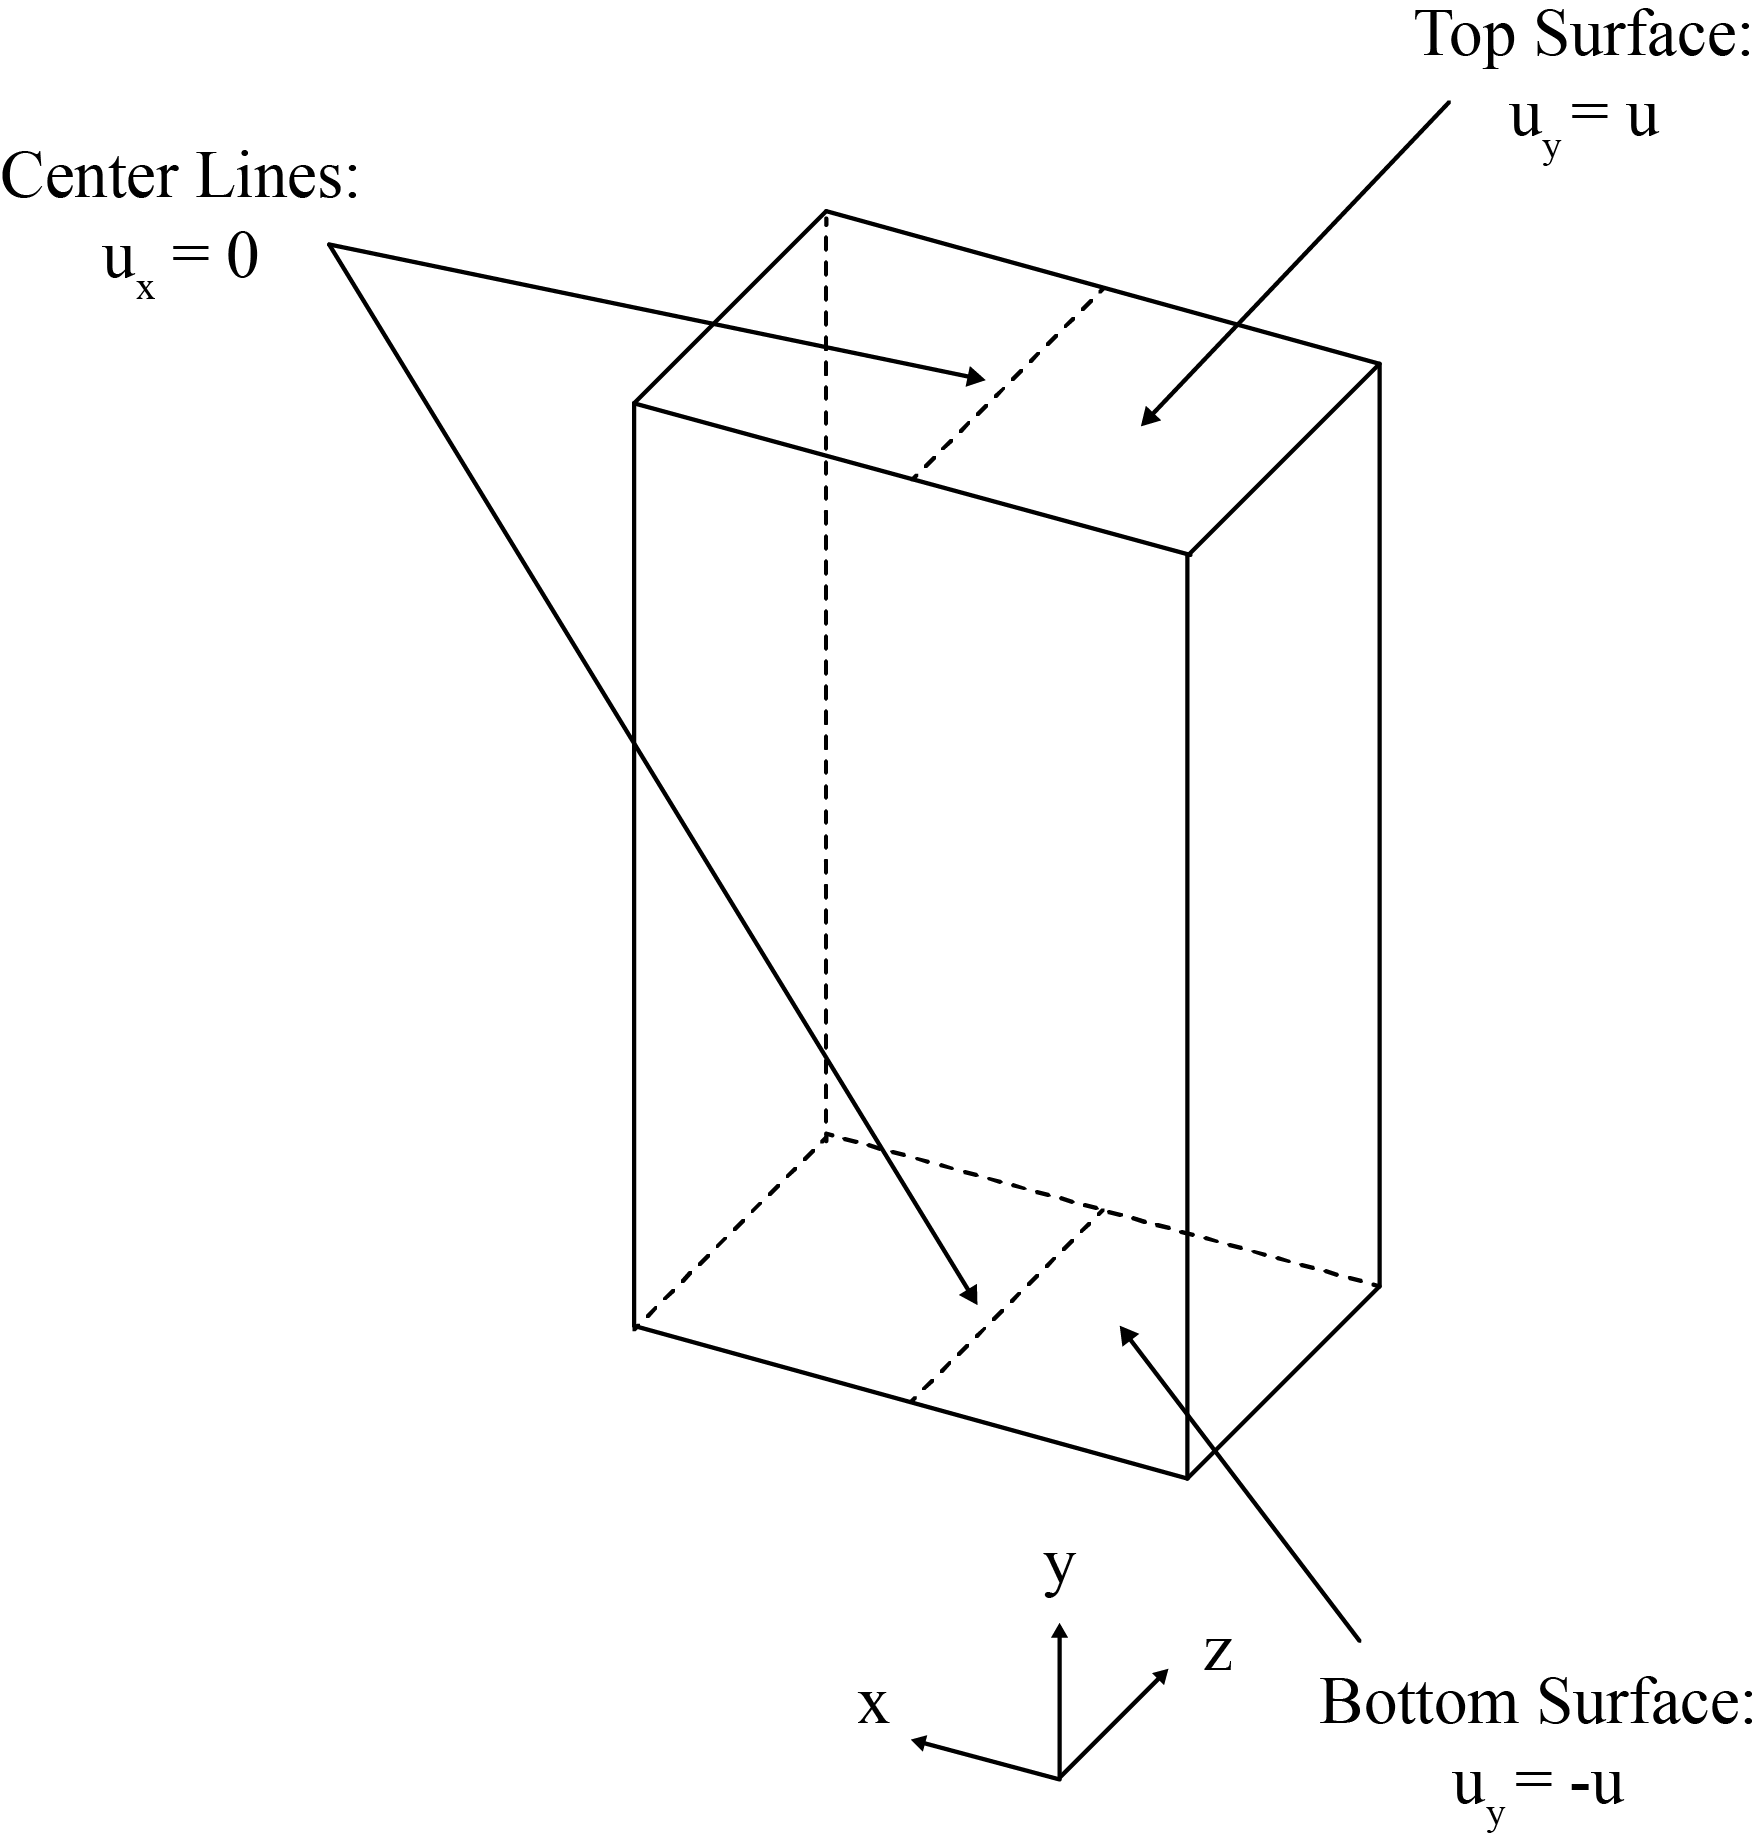
\includegraphics[width=4in]{geometry_figures/BCs.png} }}%
    \qquad
    \subfloat[\centering Model geometry]{{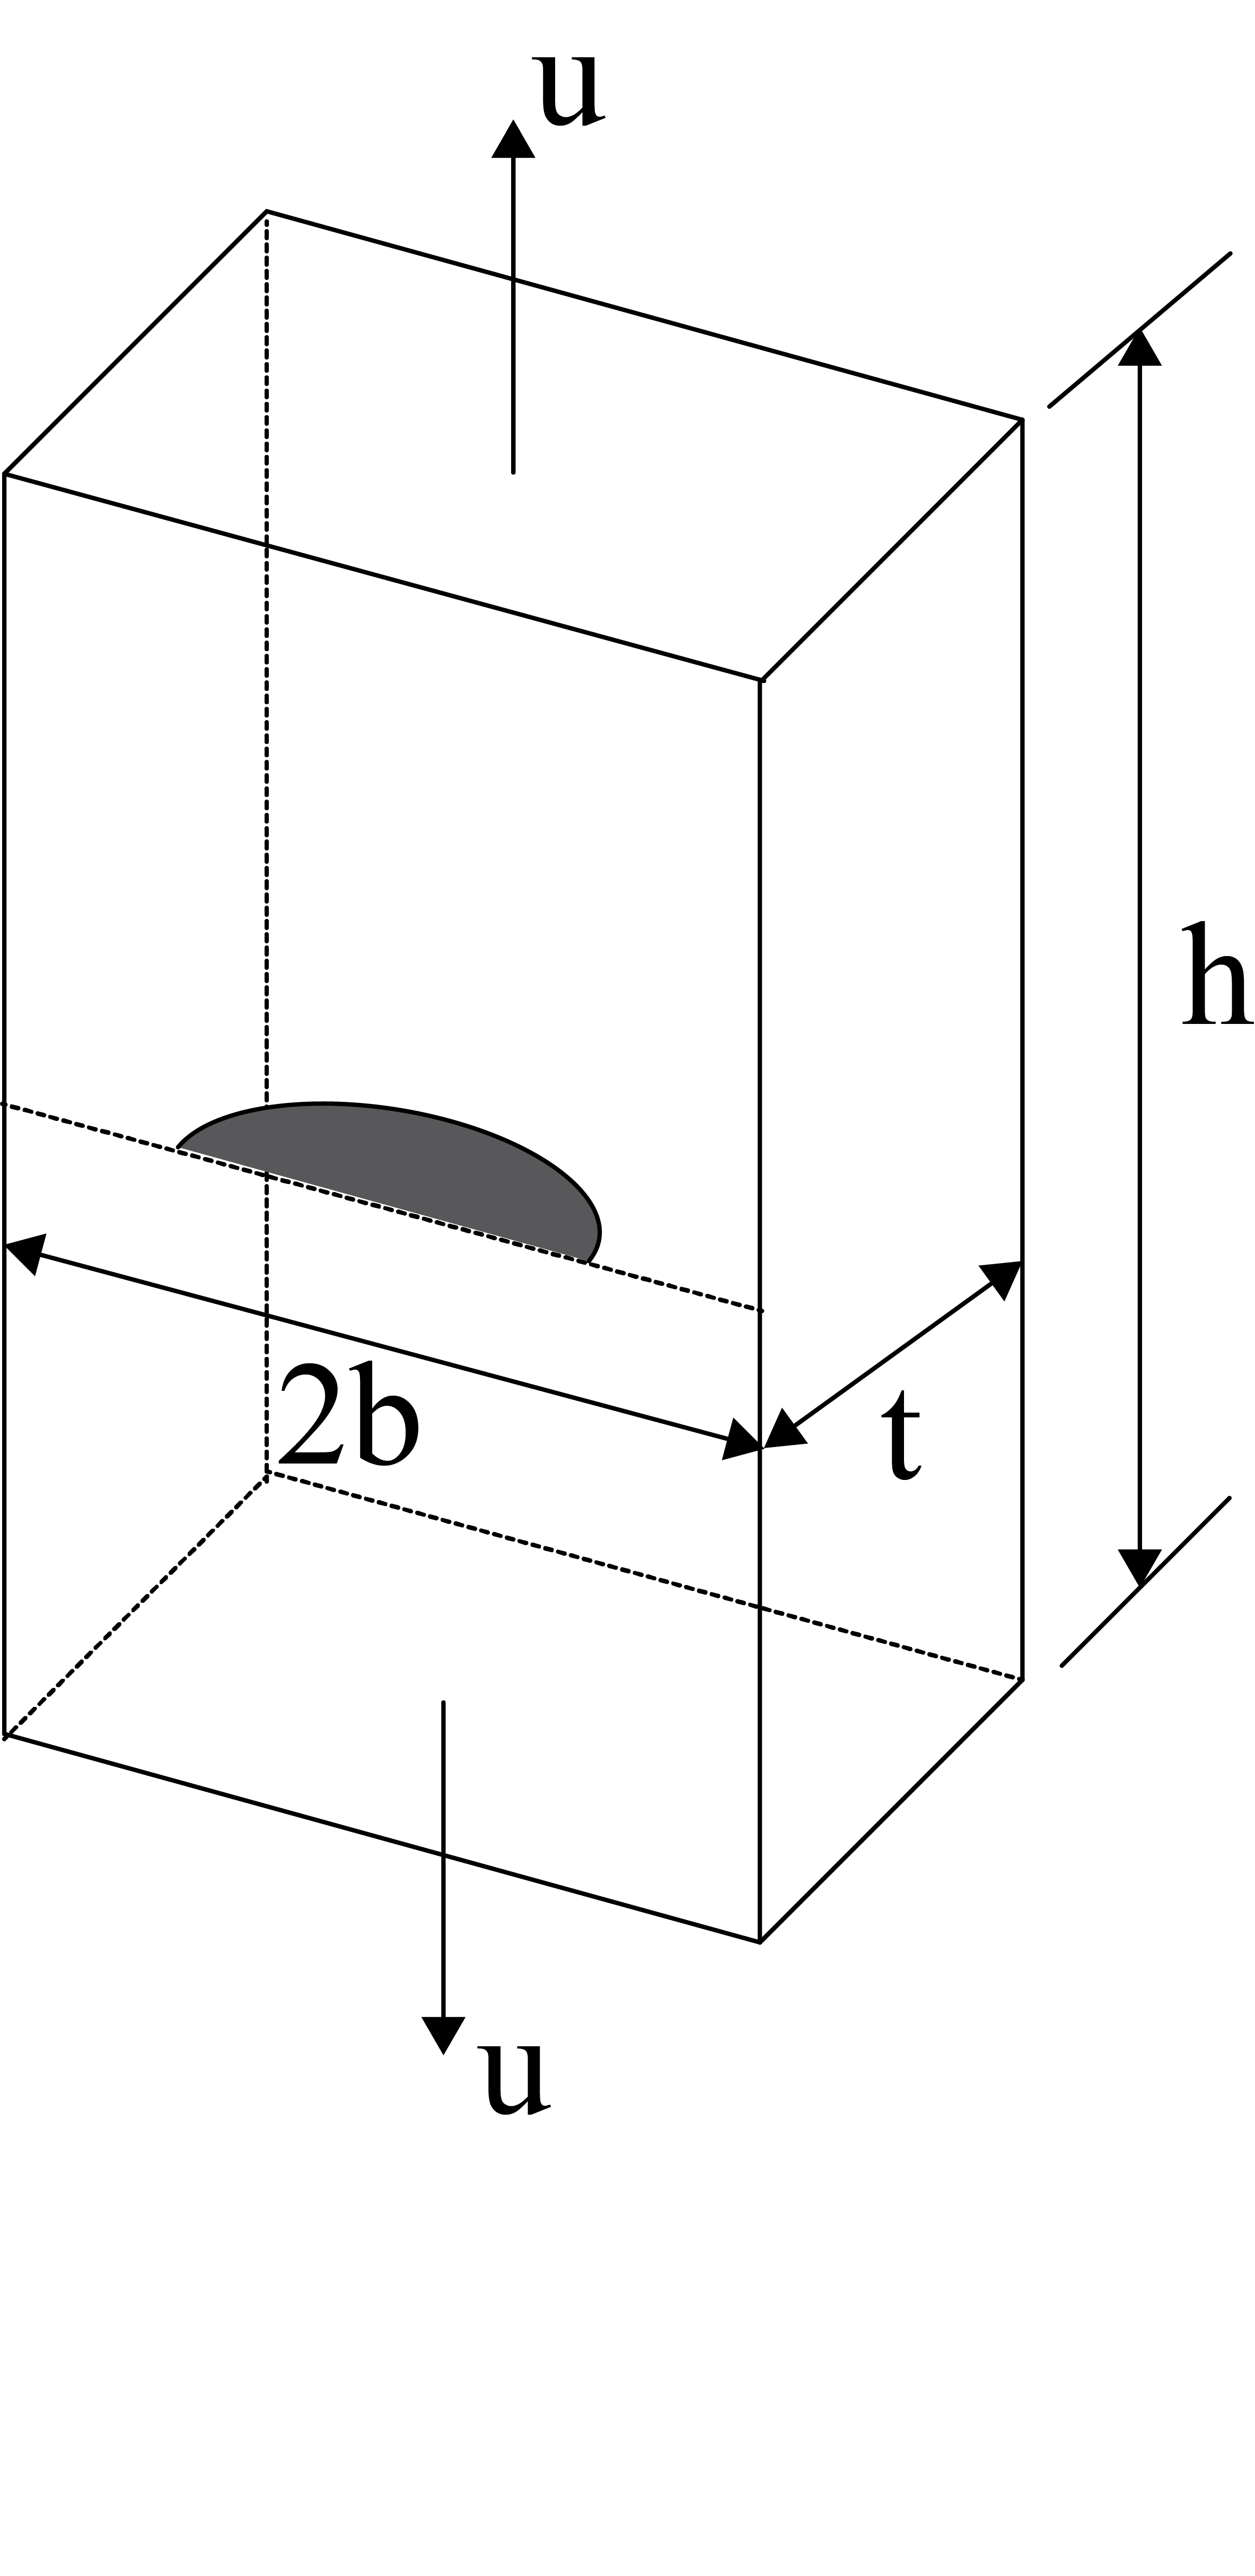
\includegraphics[width=2in]{geometry_figures/Geom.png} }}%
    \caption{(a) Top and bottom surfaces with displacement in $+y$ and $-y$ respectively. The center lines of the top and bottom faces are held $0$ in $x$. (b) Model geometry plate hight: $h$, plate width: $2b$, and plate thickness: $t$.}%
    \label{fig:model_params}%
\end{figure}

\begin{figure}%
    \centering
    \subfloat[\centering Crack dimensions]{{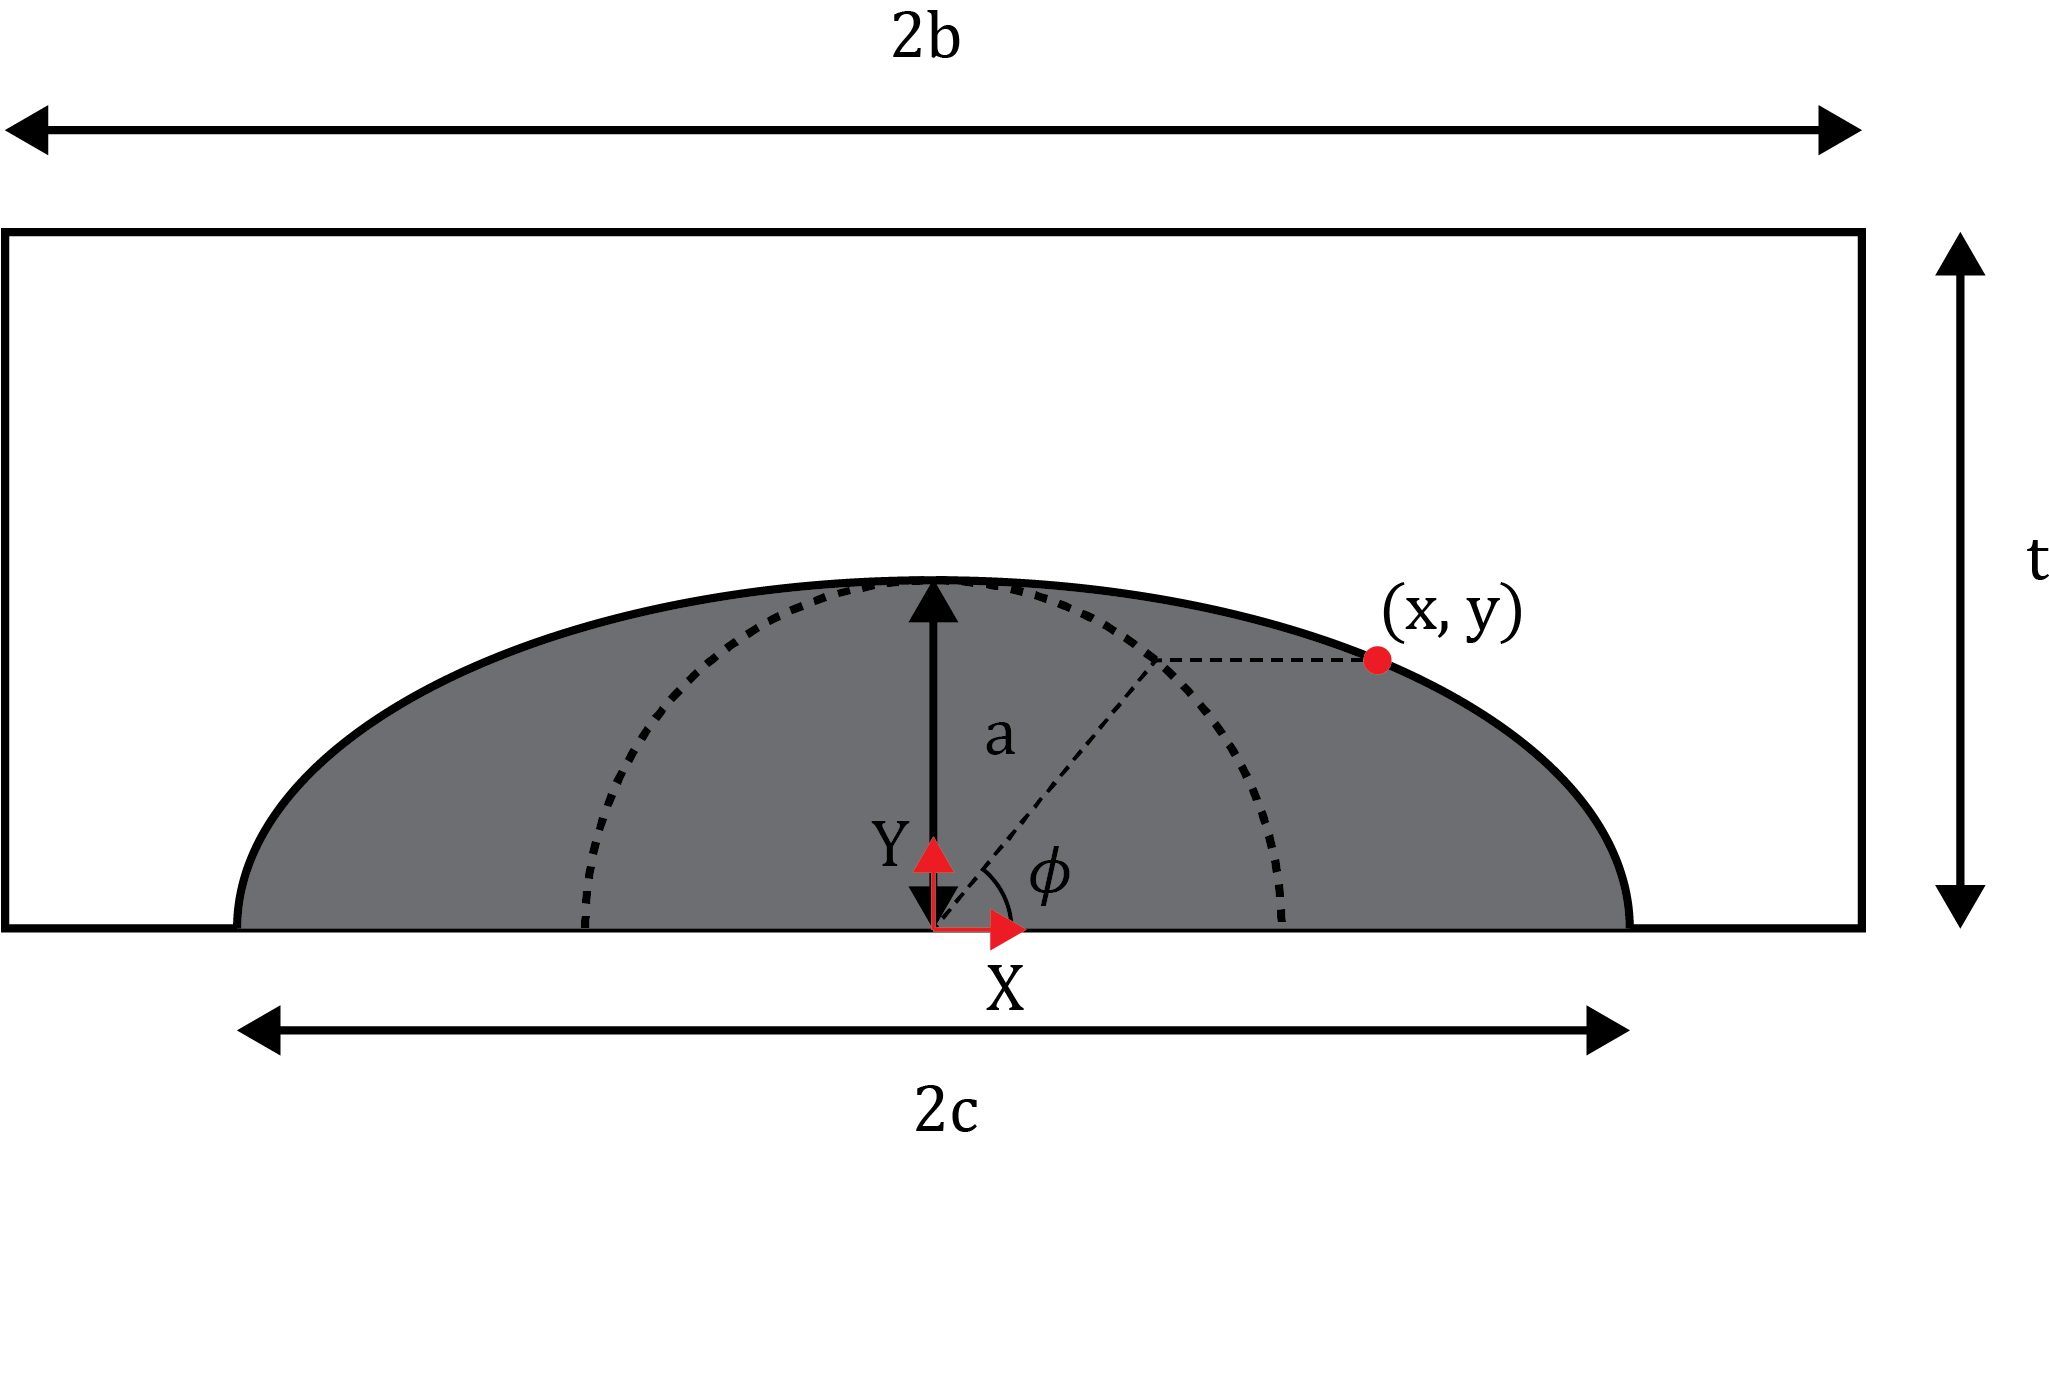
\includegraphics[width=3in]{geometry_figures/params.png} }}%
    \qquad
    \subfloat[\centering Ellipse dimensions]{{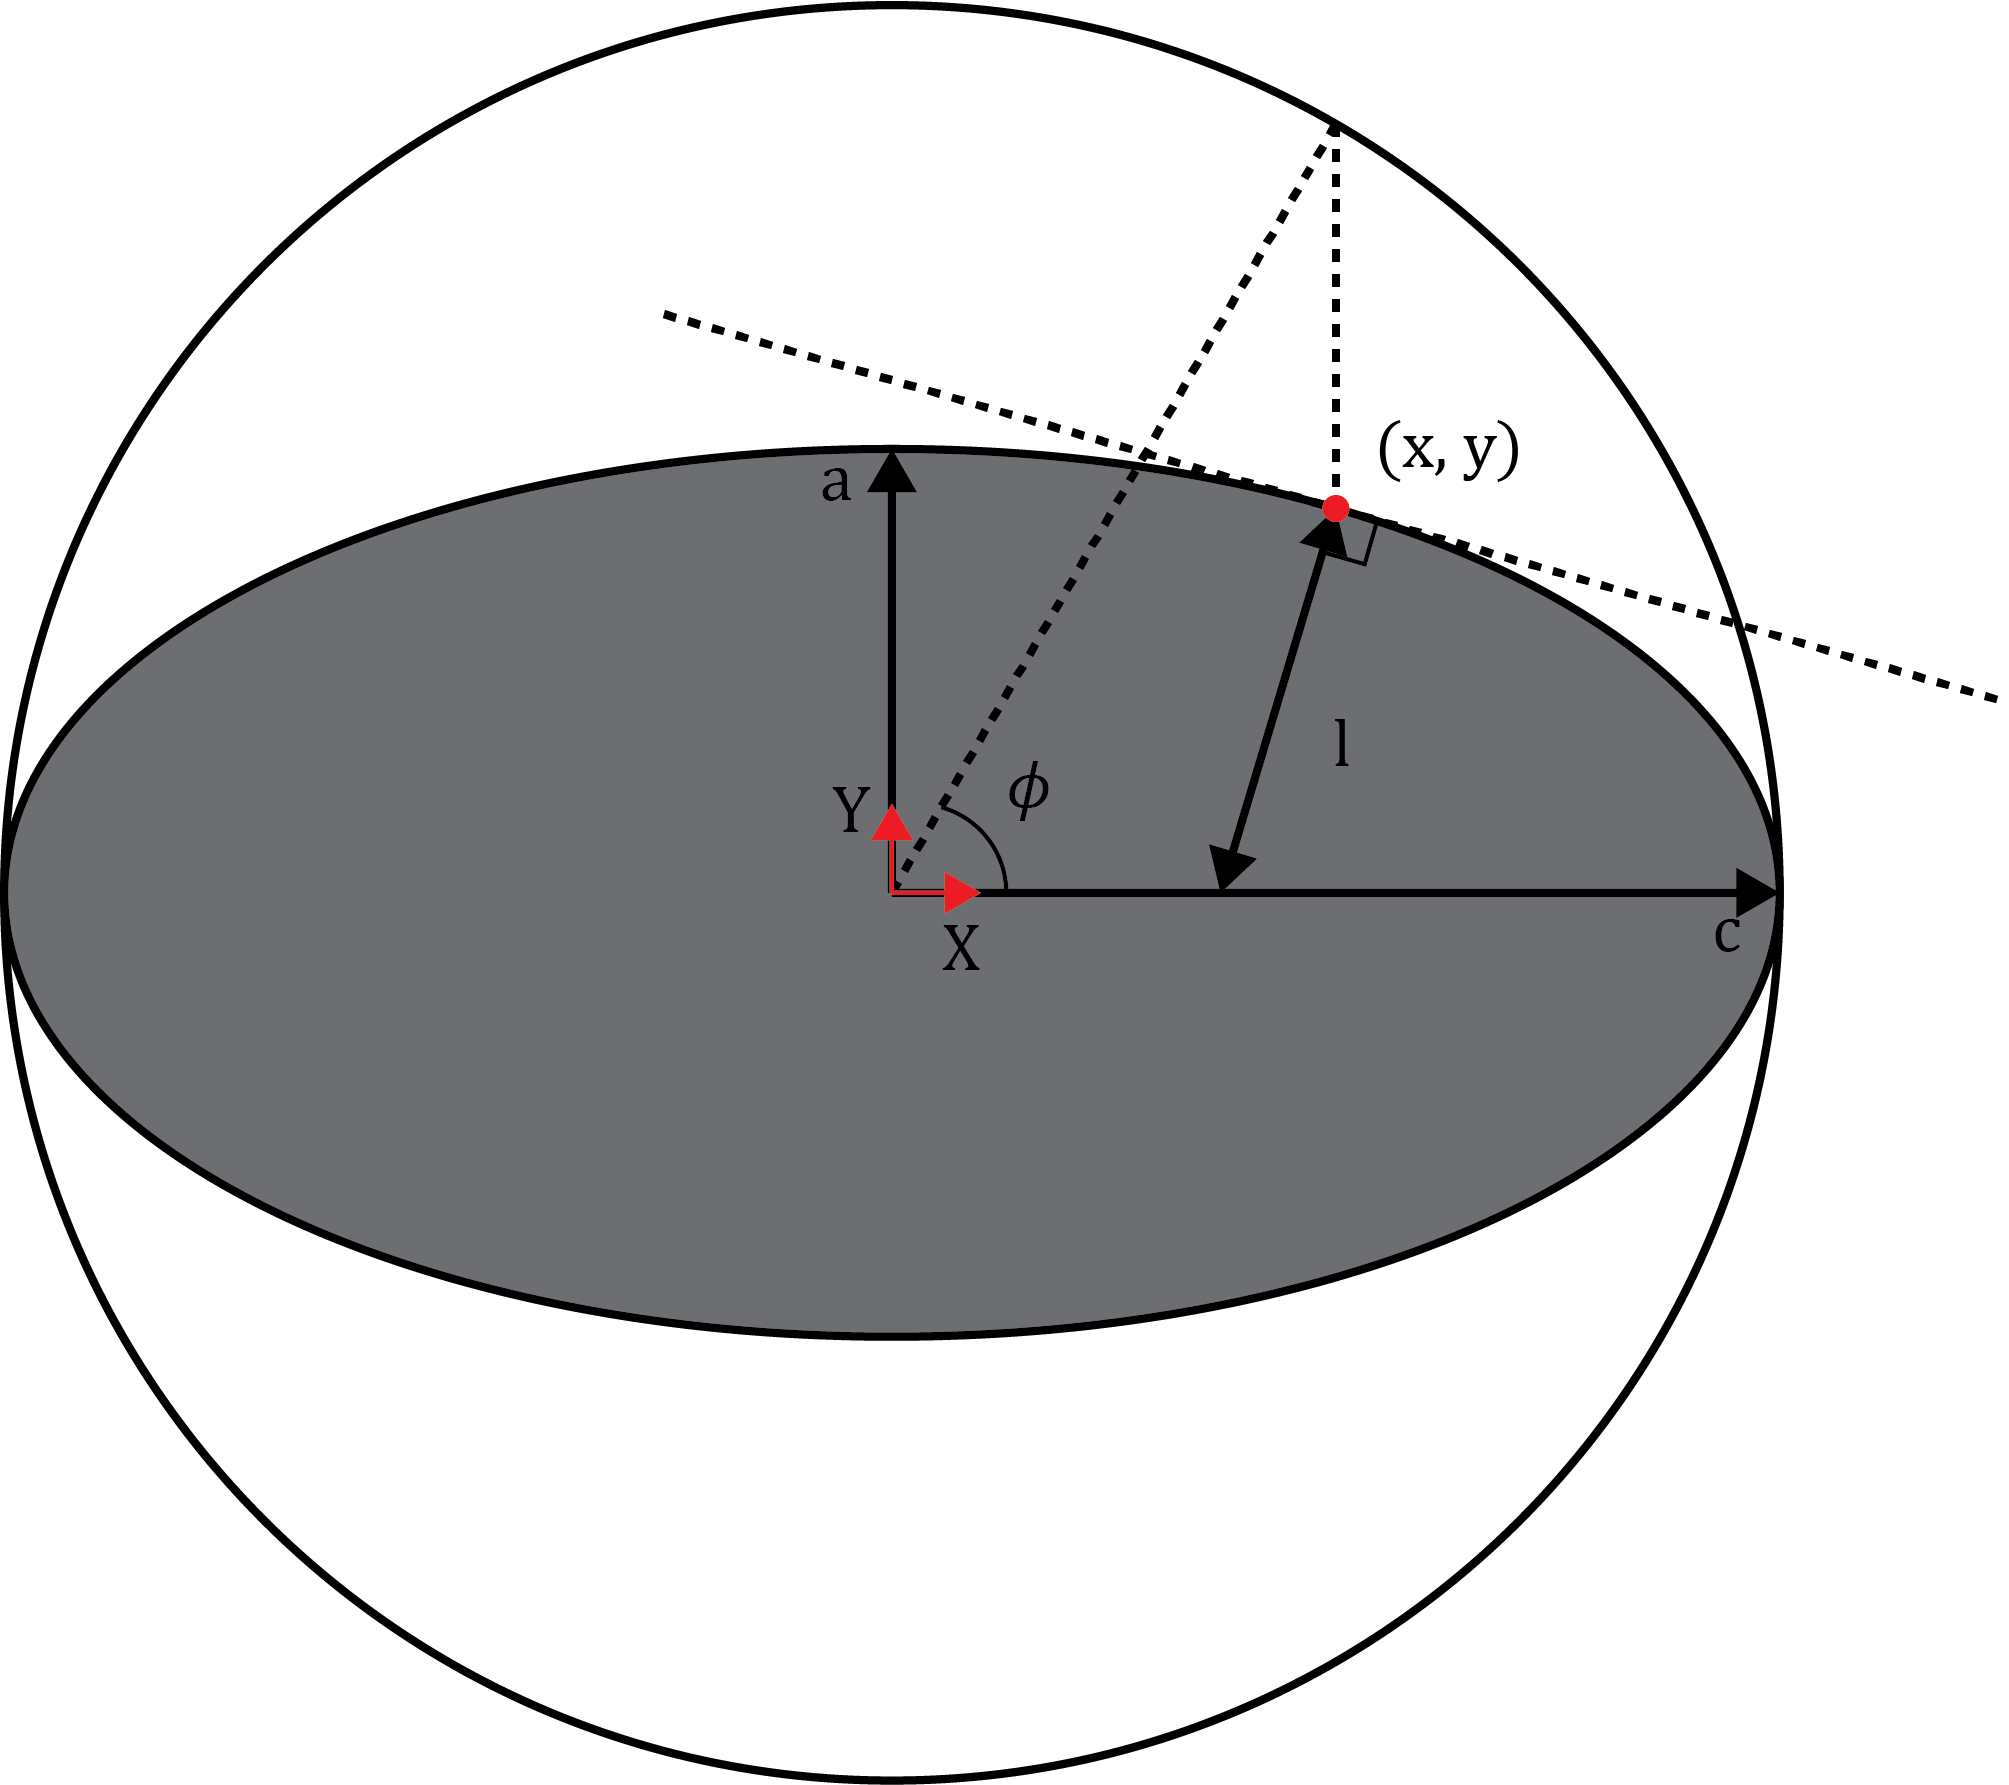
\includegraphics[width=3in]{geometry_figures/Ellipse.png} }}%
    \caption{(a) Crack pameters with $a$ being the crack depth and $2c$ being the surface crack length. (b) $\phi$ is defined by the angle to the enscribed circle projected to the ellipse. $l$ is defined as the distance perpendicular to the tangent line from the point of interest to the nearest axis.}%
    \label{fig:crack_params}%
\end{figure}


\begin{figure}%
    \centering
    \subfloat[\centering Convergence of $h/t$]{{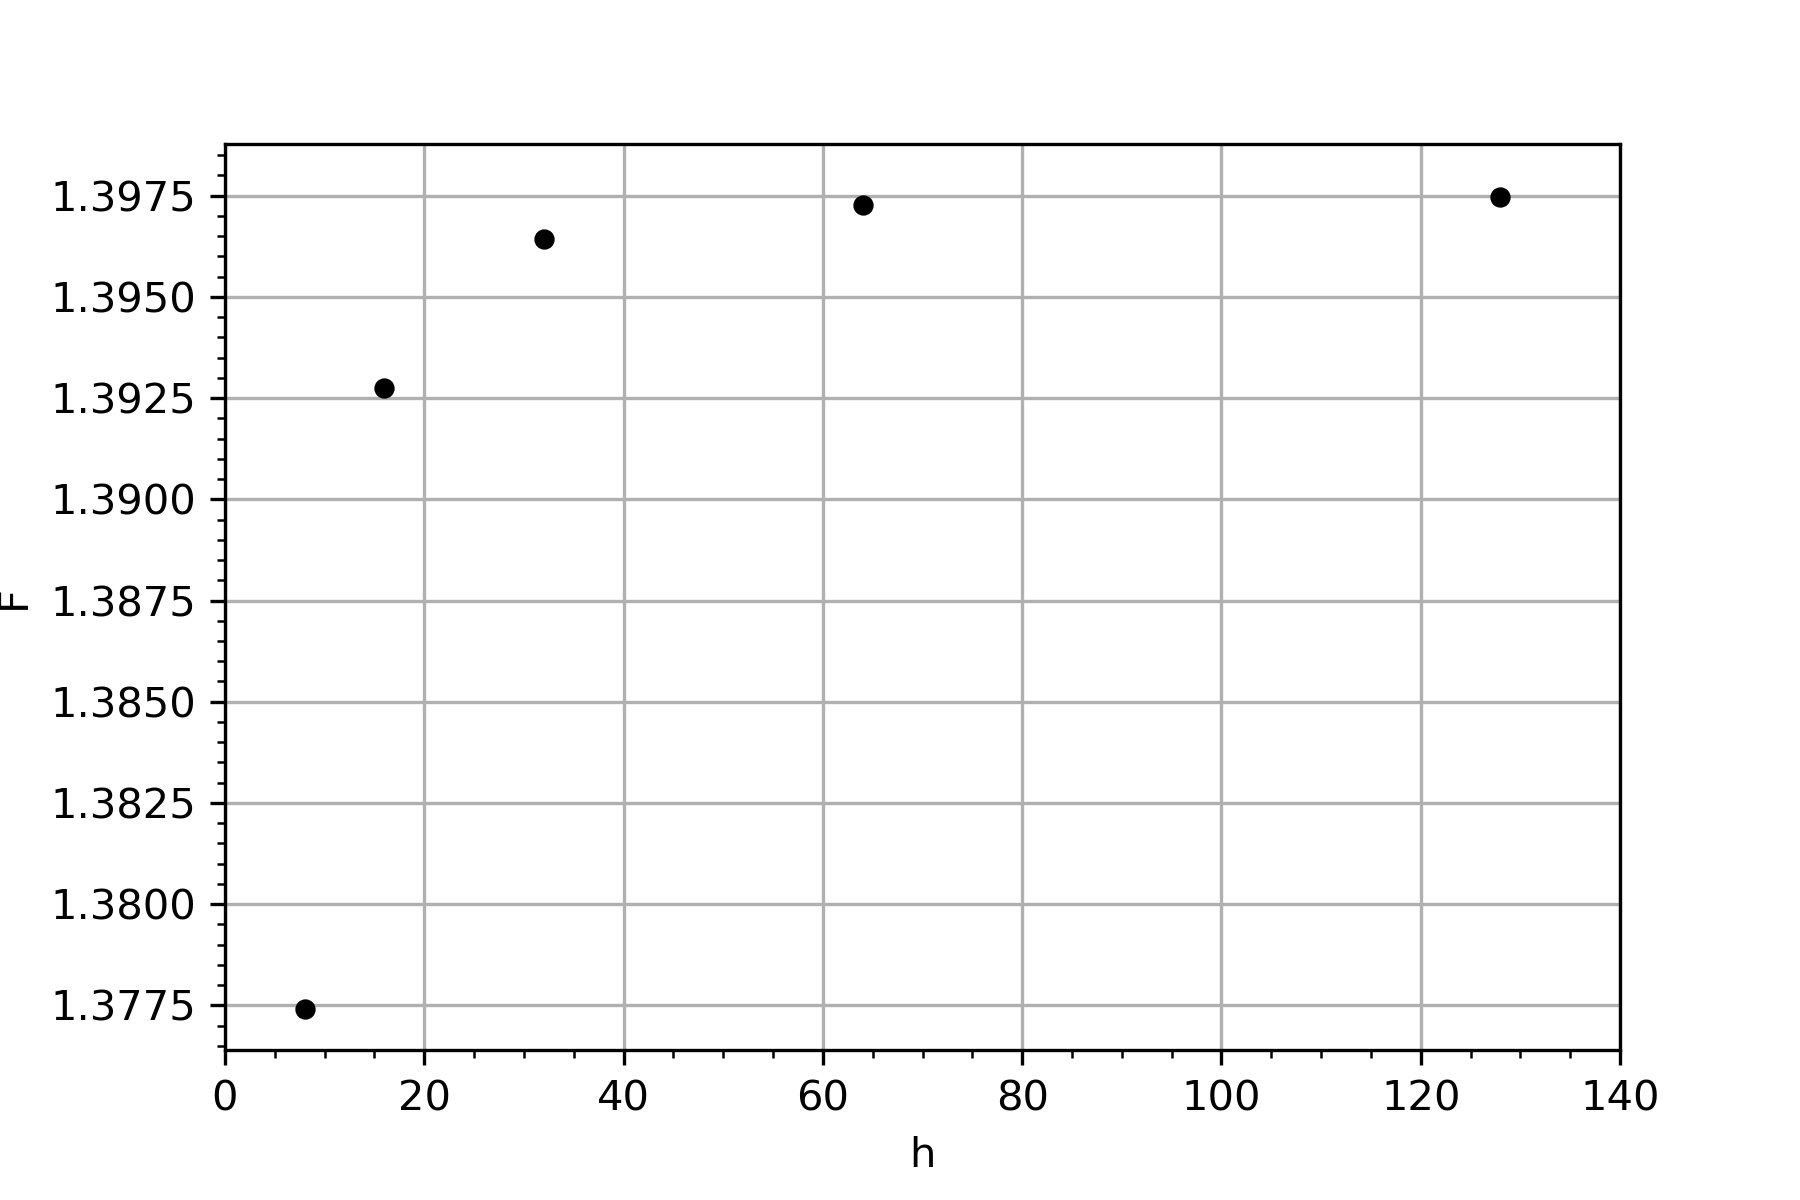
\includegraphics[width=3in]{Figures/h_convergence.png} }}%
    \qquad
    \subfloat[\centering convergence of $c/b$]{{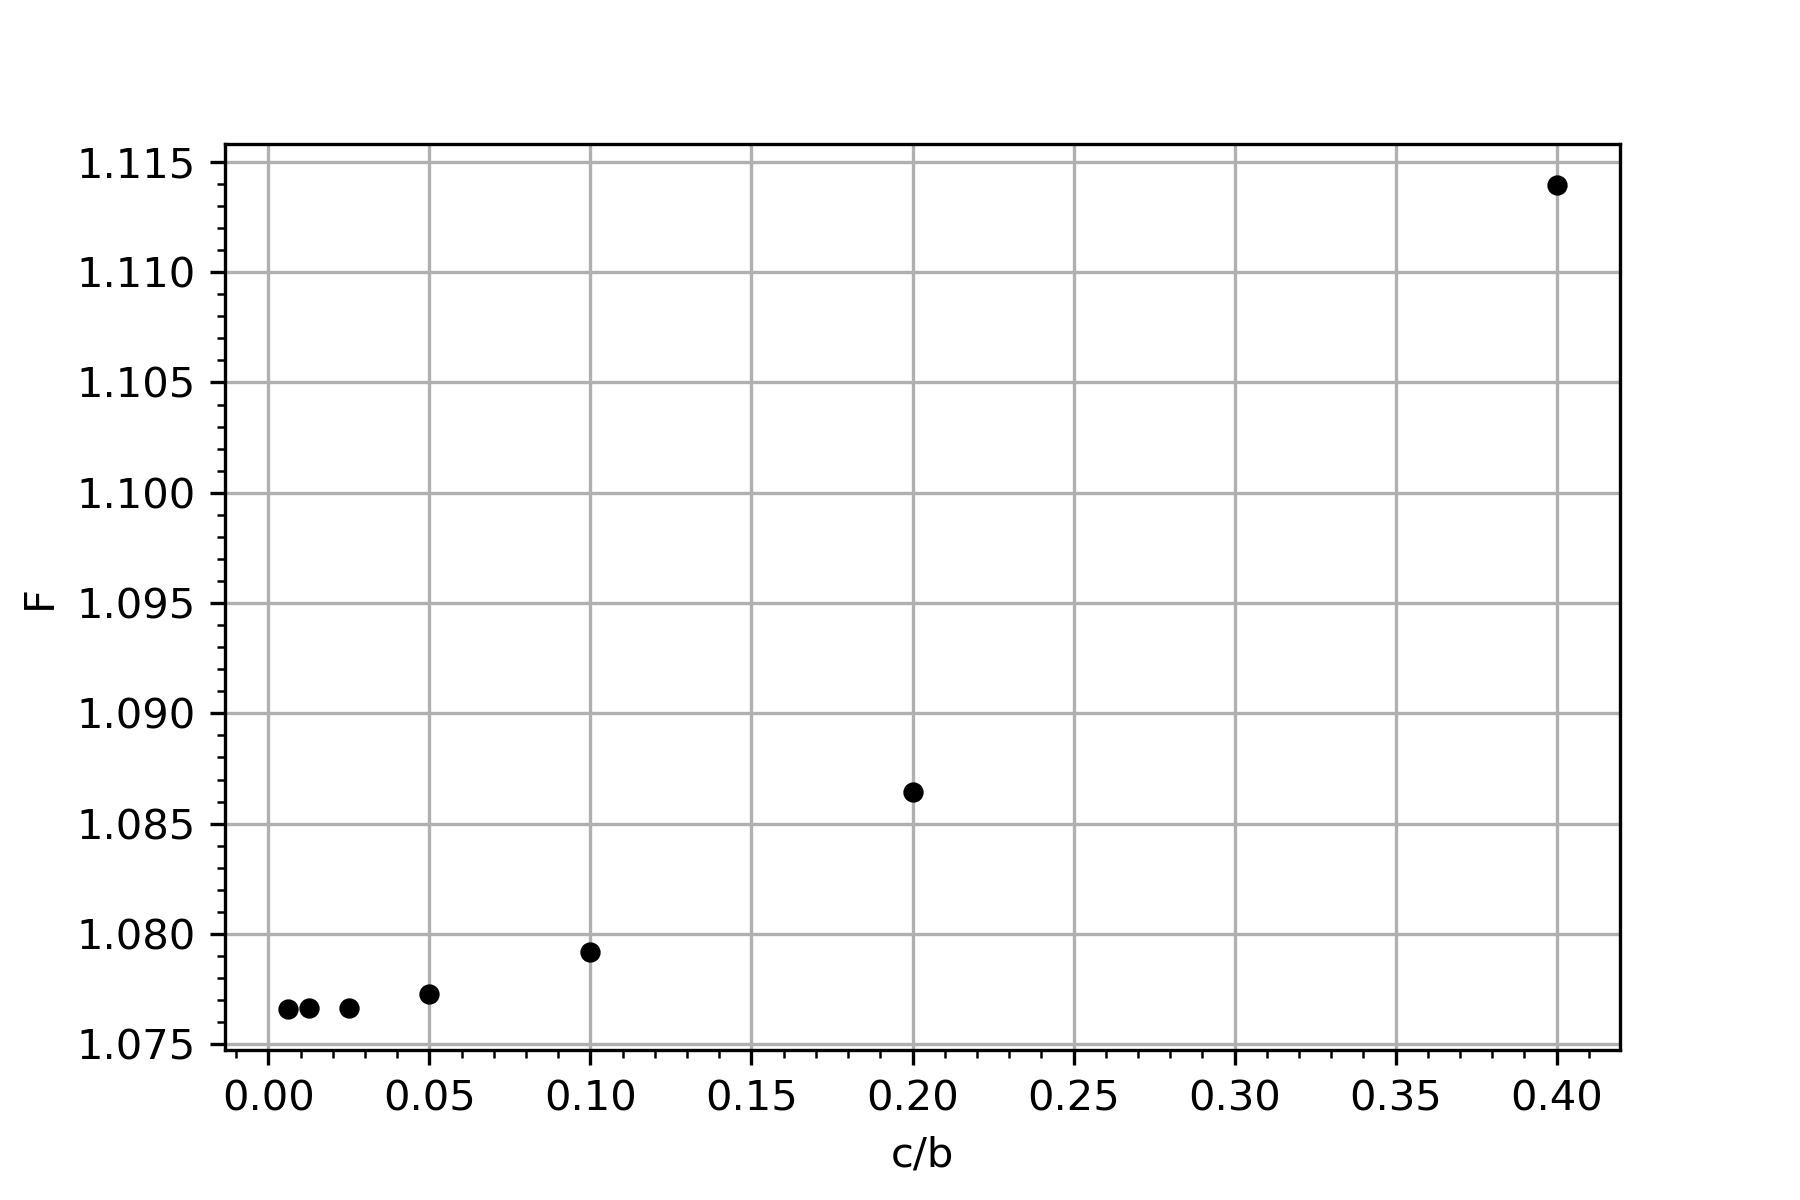
\includegraphics[width=3in]{Figures/cb_convergence.png} }}%
    \caption{(a) the convergence of $h/t$ is plotted using the mean boundary correction factor (b) The convergence of $c/b$ is plotted using the mean boundary correction factor.}%
    \label{fig:convergence_plots}%
\end{figure}


\begin{figure}
    \centering
    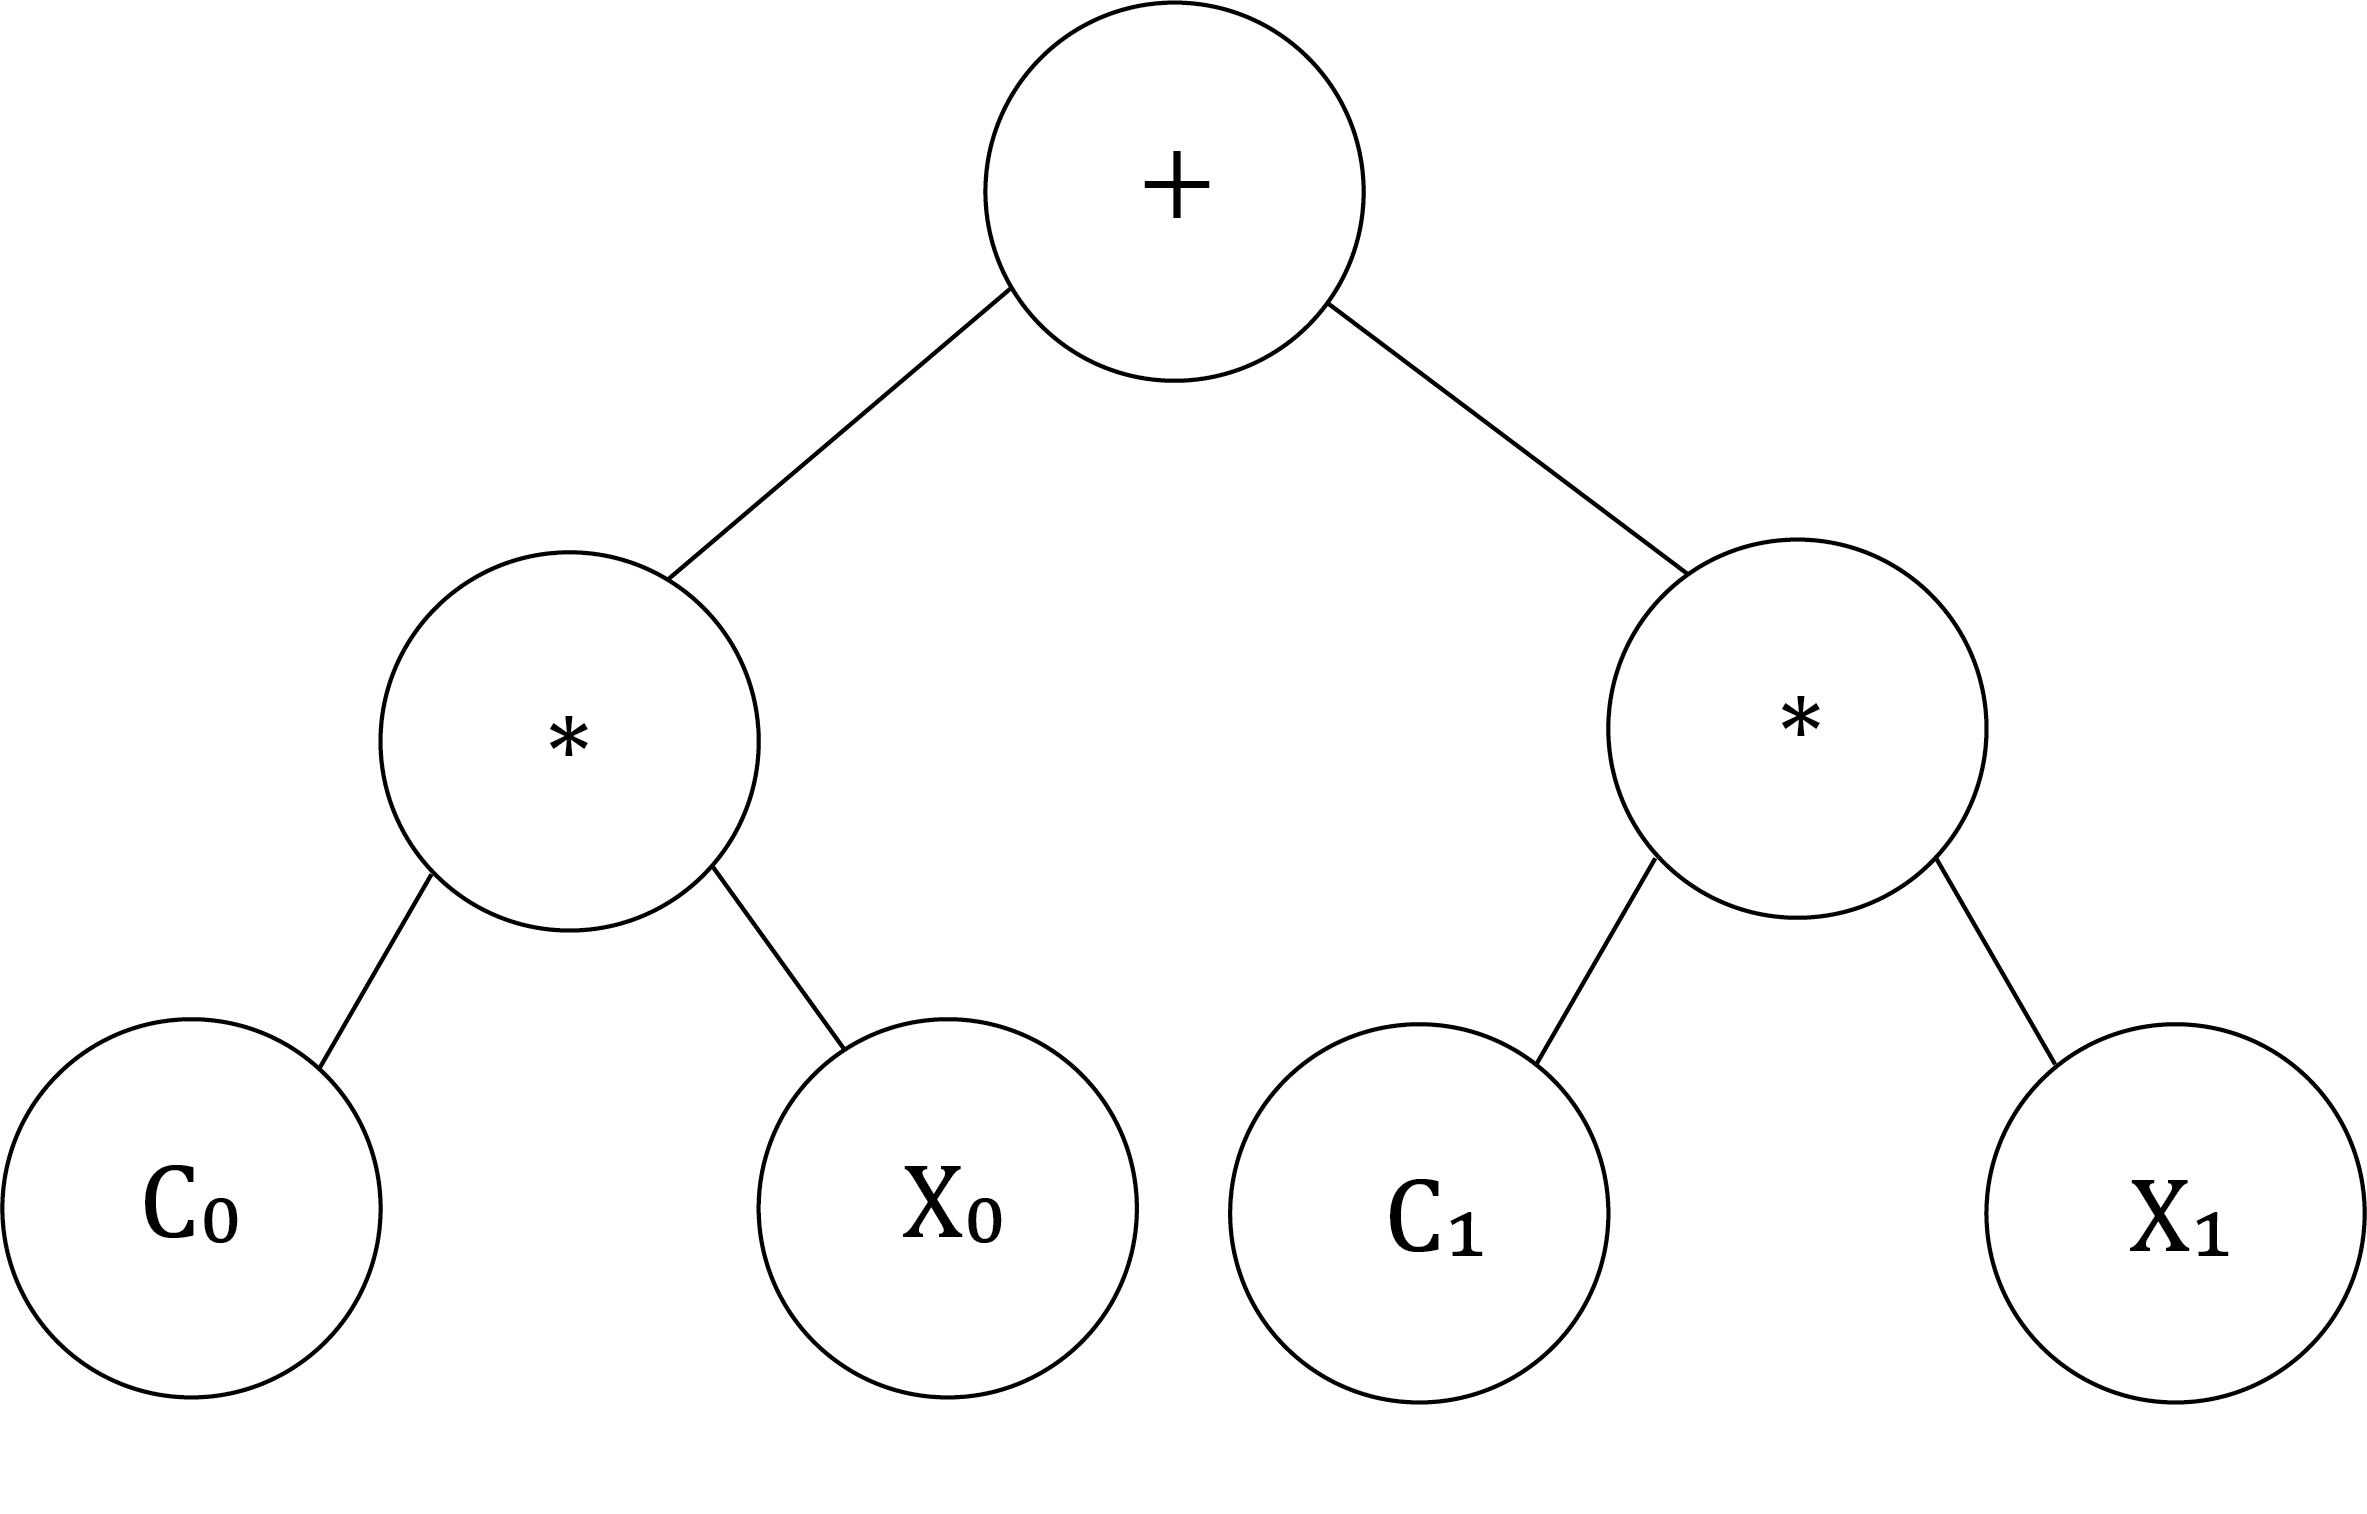
\includegraphics[width=4in]{geometry_figures/agraph.png}
    \label{fig:agraph}
    \caption{Example Agraph for for equation; $C_0 X_0 + C_1 X_1$, where the complexity is the sum of the nodes in this case 7.} 
\end{figure}


\begin{figure}%
    \centering
    \subfloat[\centering Distributions of error]{{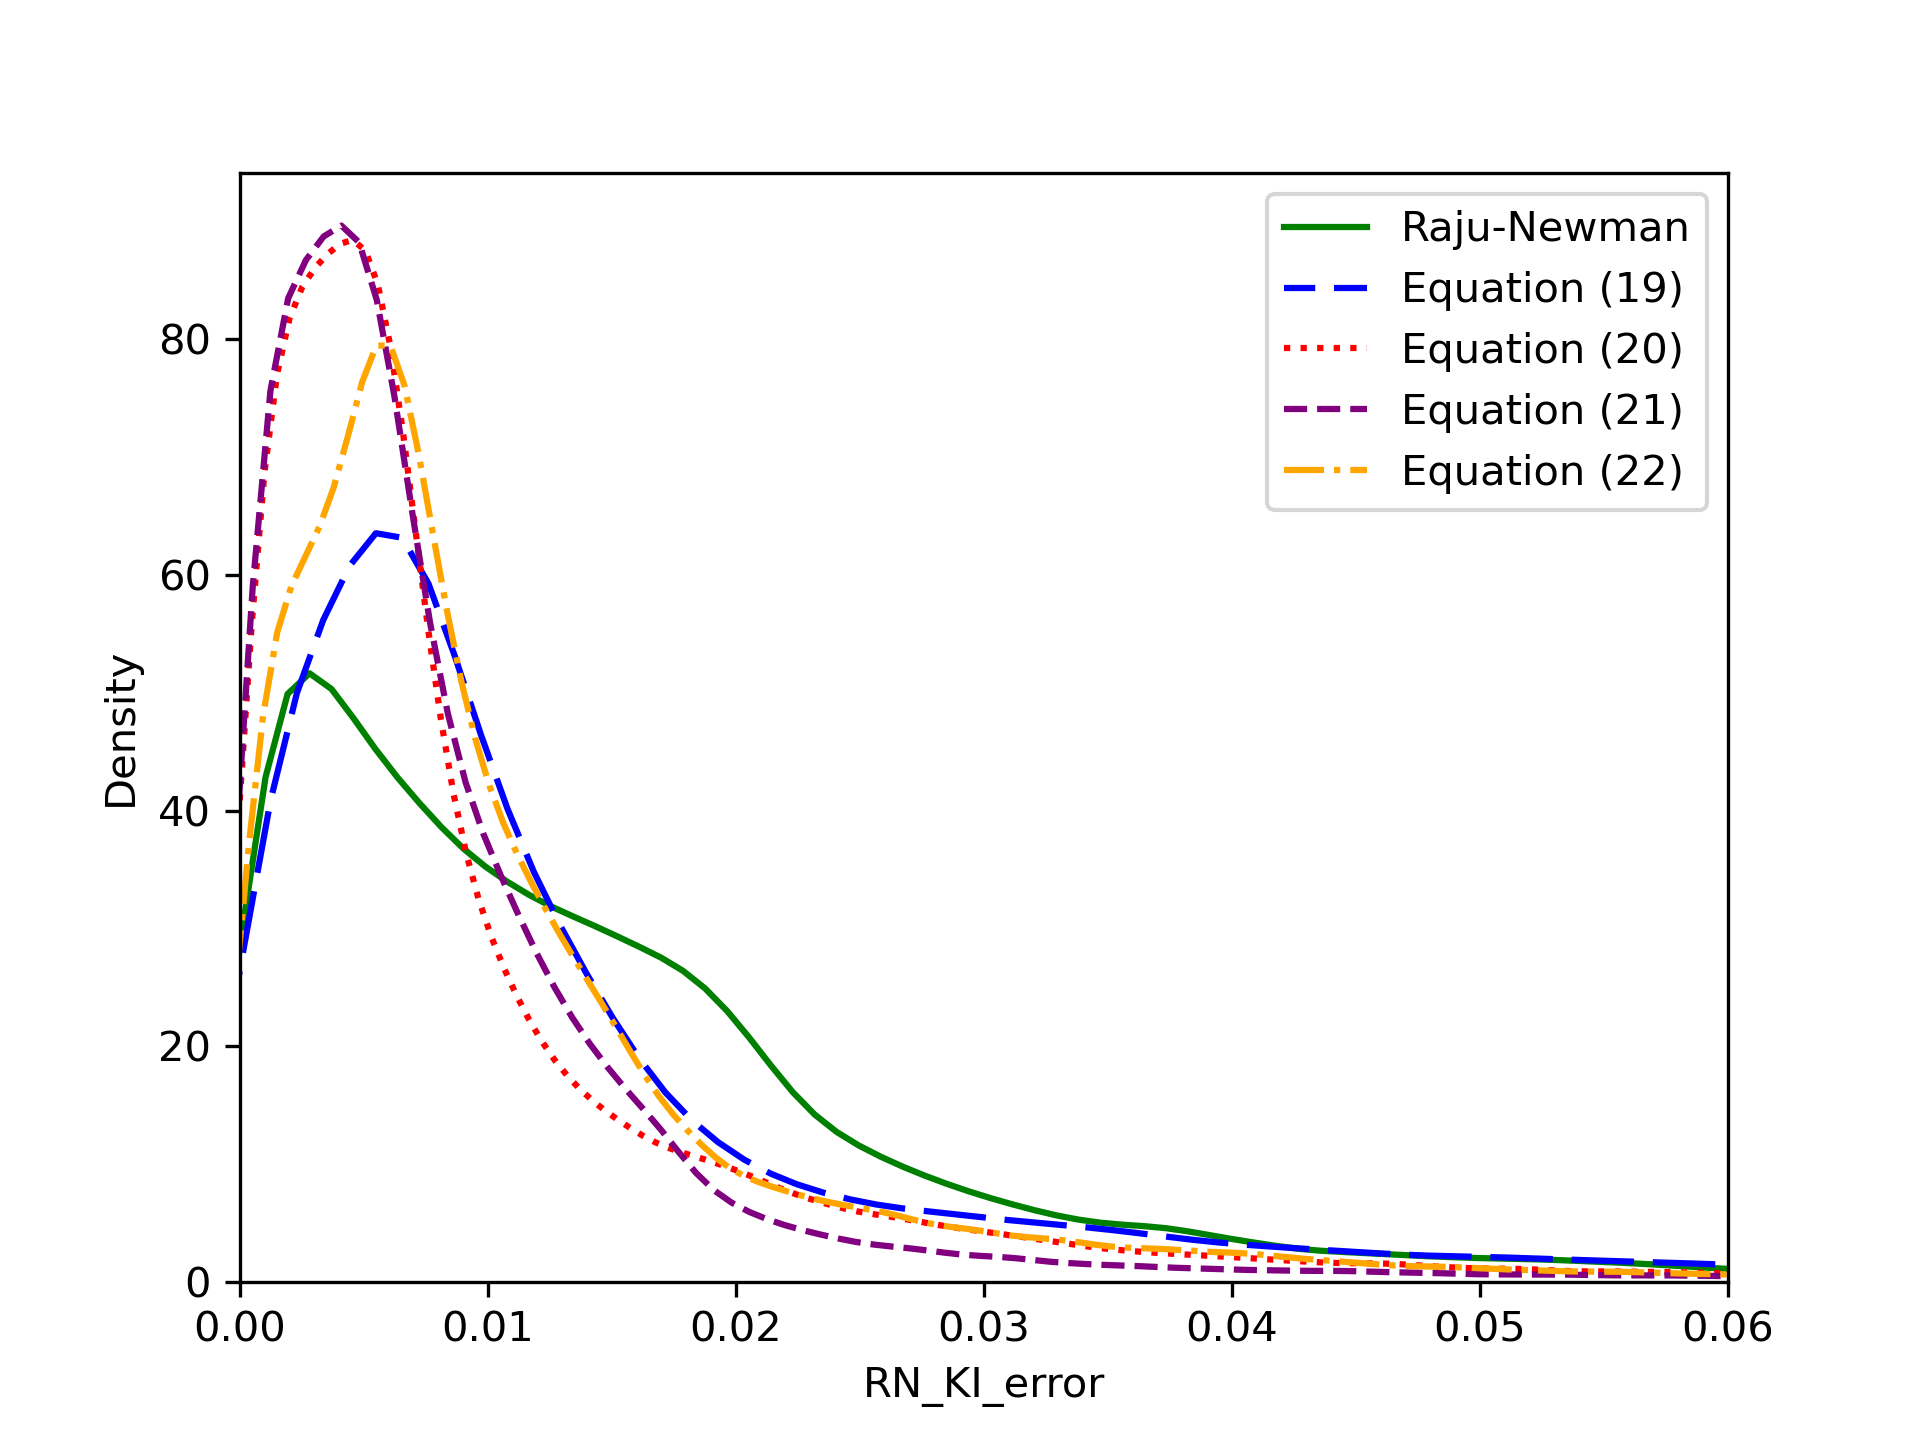
\includegraphics[width=3in]{Figures/kde_plot.png} }}%
    \qquad
    \subfloat[\centering Parity plots]{{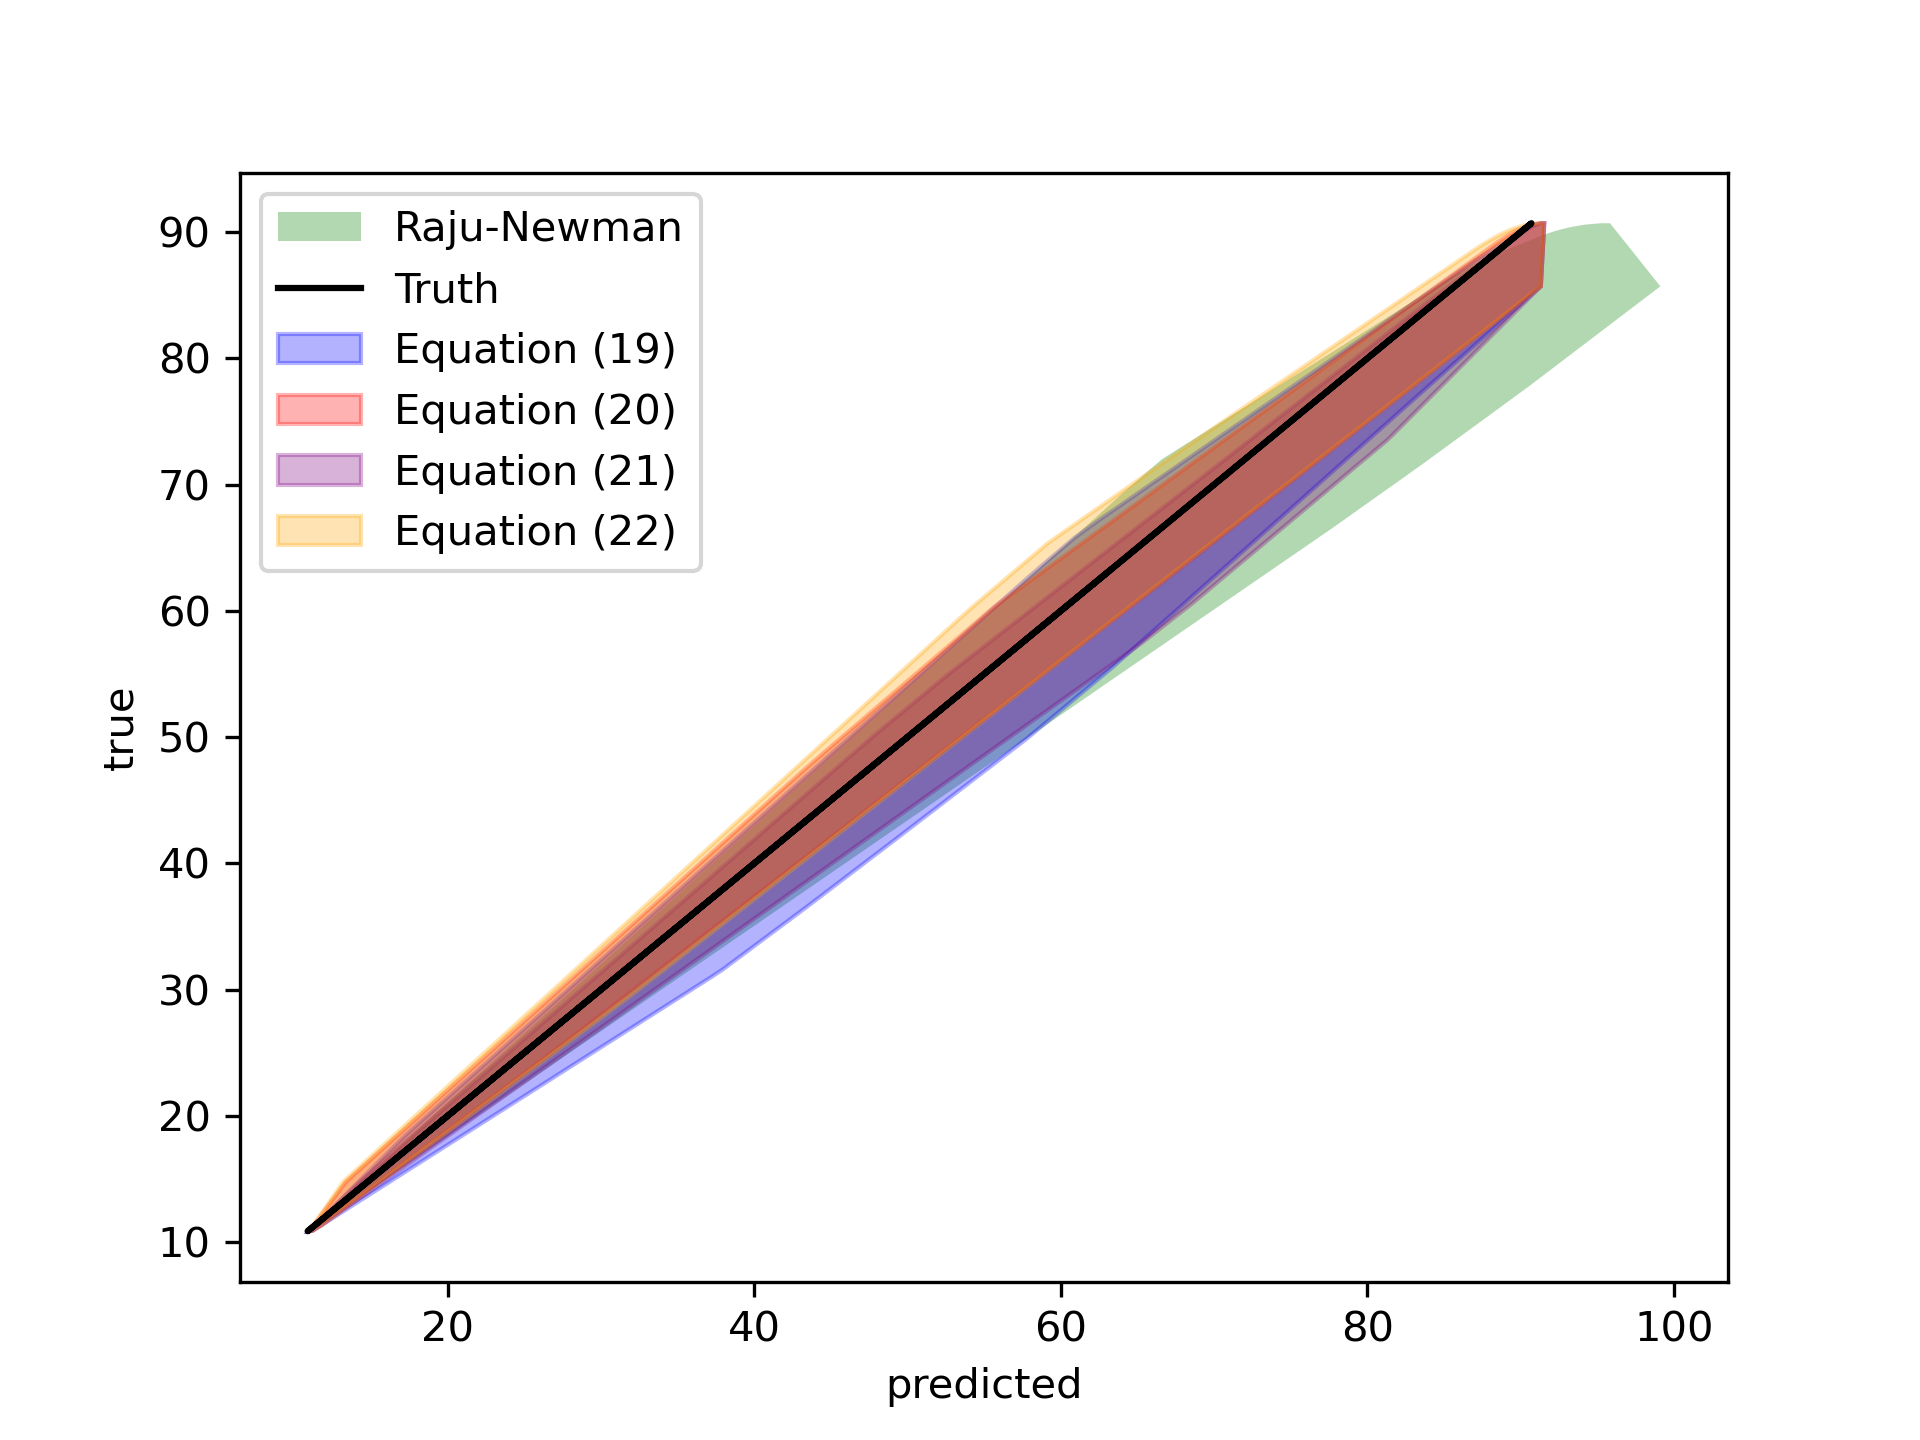
\includegraphics[width=3in]{Figures/parity_plot.png} }}%
    \caption{(a) Density plot for the errors of each of the equations. (b) Parity plot with each of the different equations.}%
    \label{fig:error_plots}%
\end{figure}


\begin{figure}
    \centering
    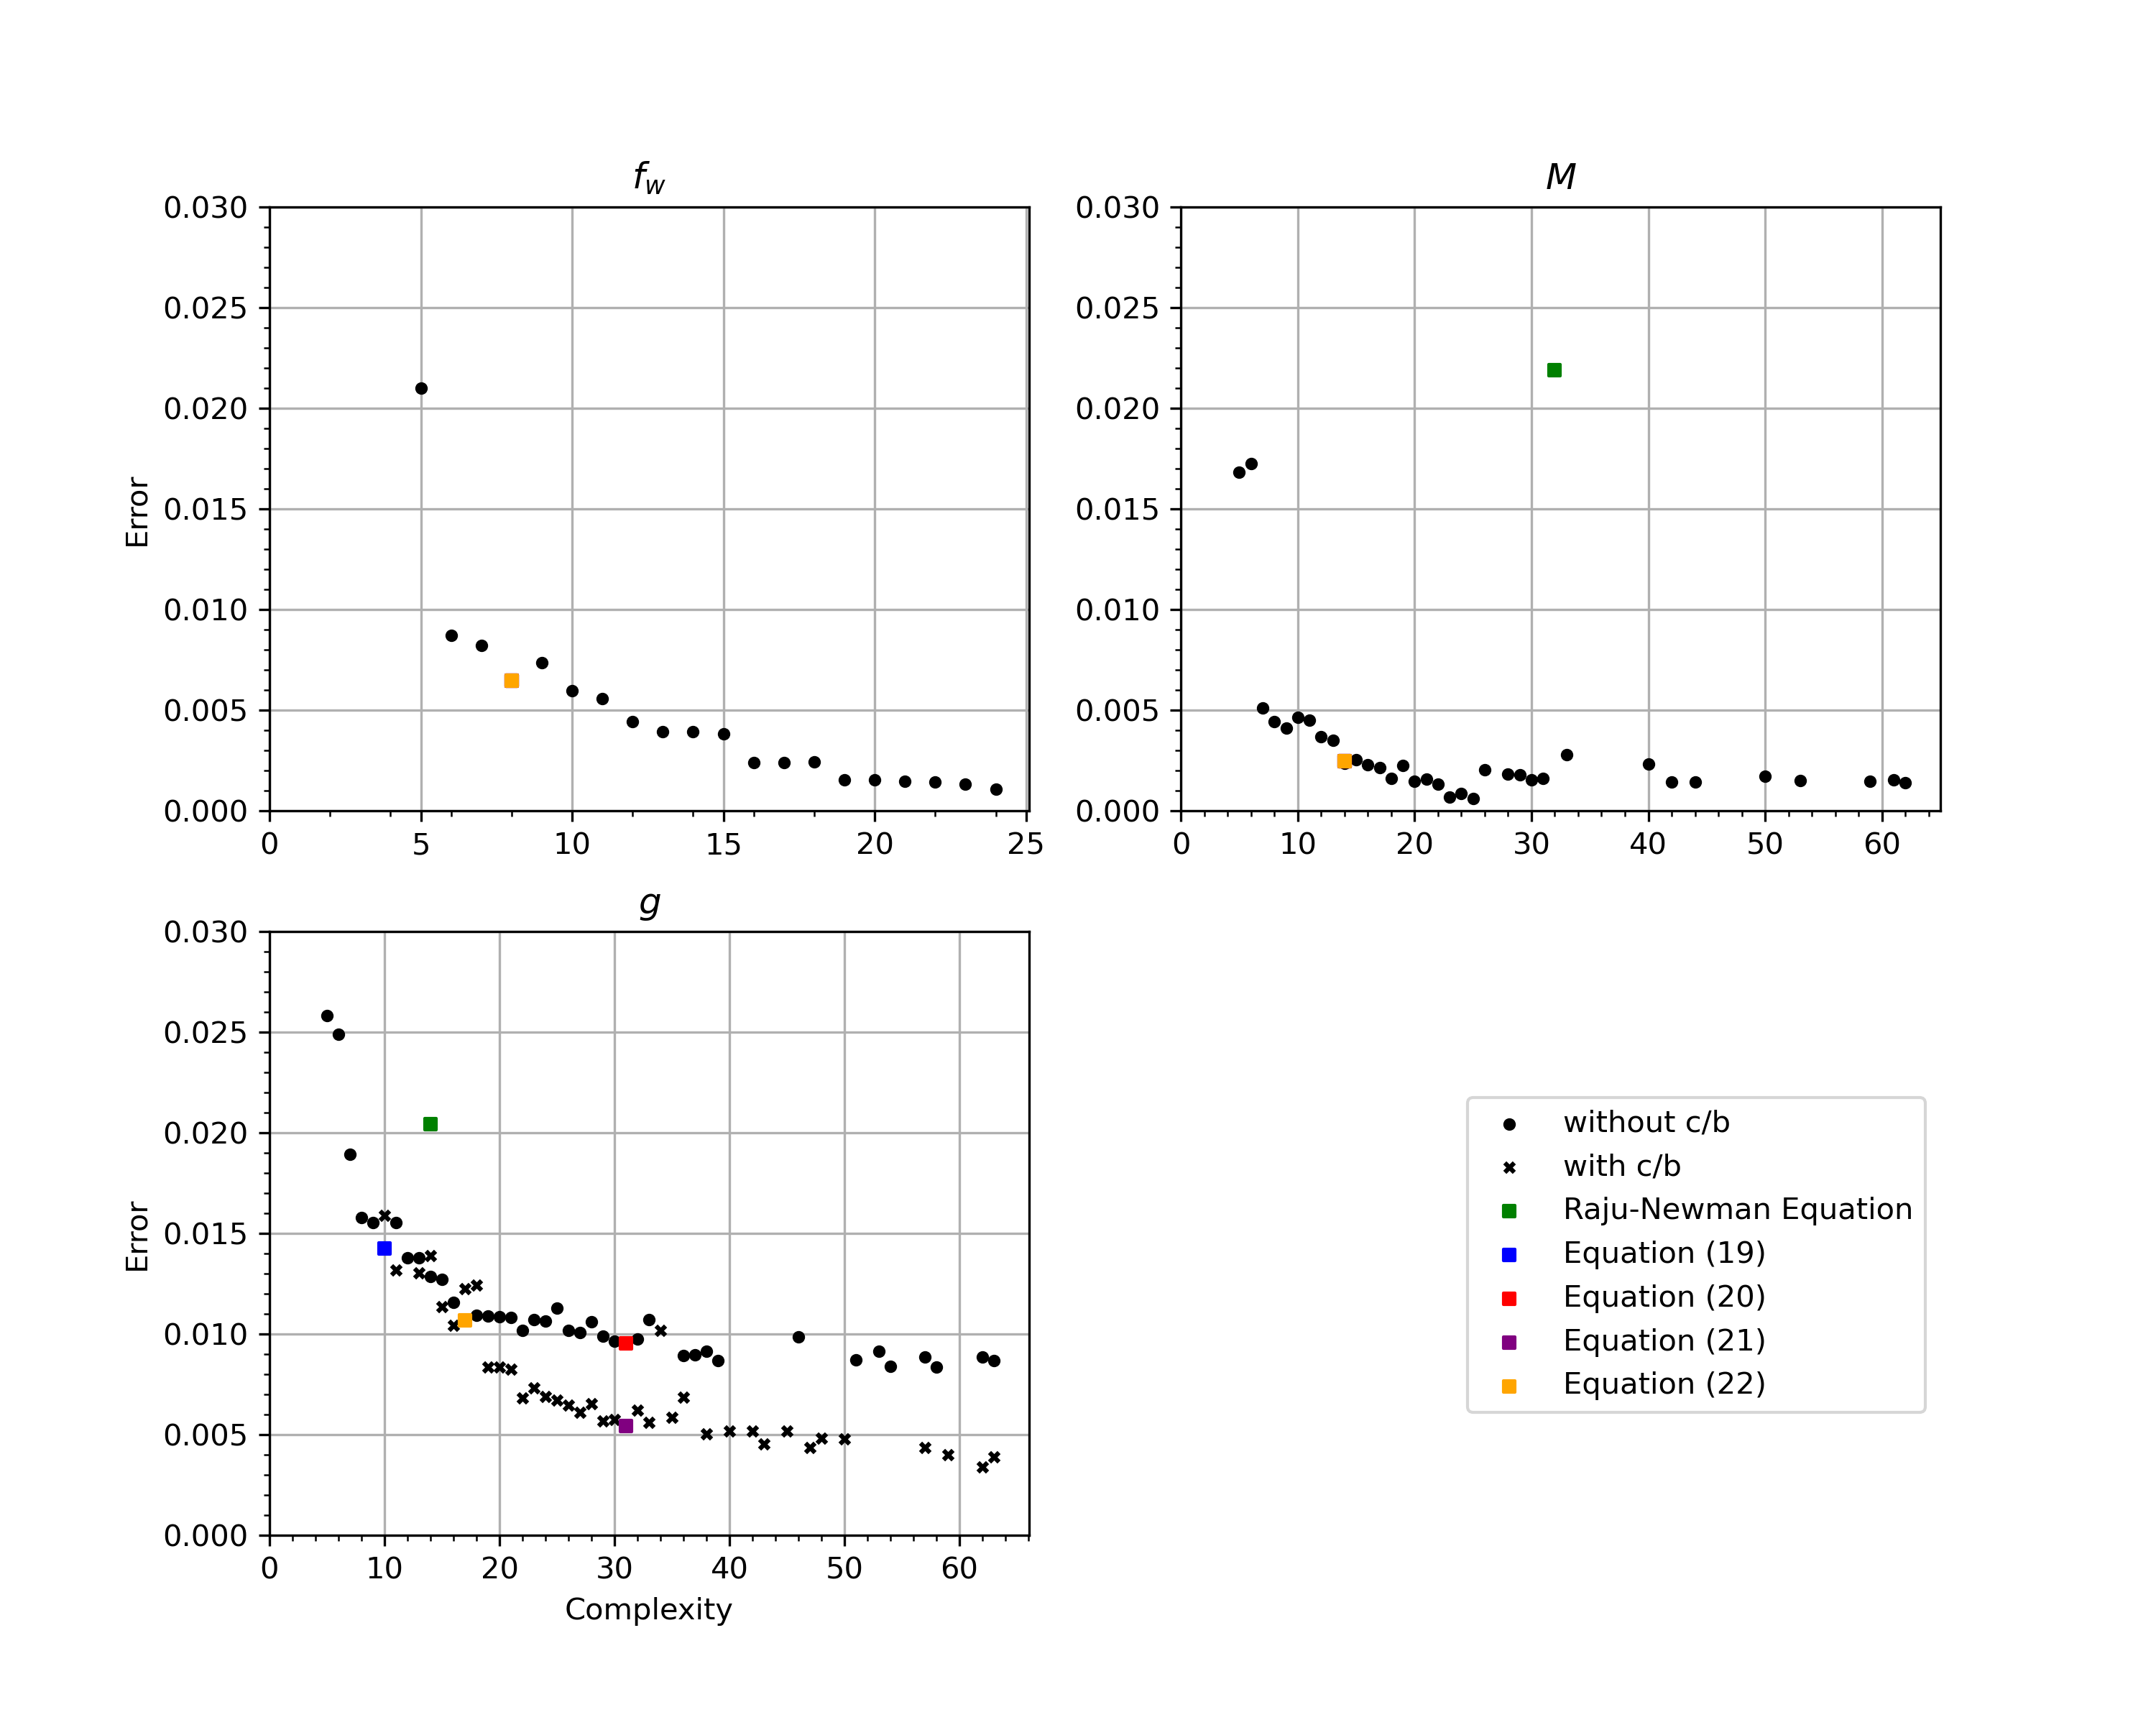
\includegraphics[width=6in]{Figures/perato_front.png}
    \label{fig:perato_front}
    \caption{Perato fronts for $f_w$, $M$, and $g$. $f_w$ and $M$ have the same equation for all four models. Both the perato fronts for $g$ with and without $c/b$ are shown} 
\end{figure}

\begin{figure}%
    \centering
    \subfloat[\centering Distributions of error]{{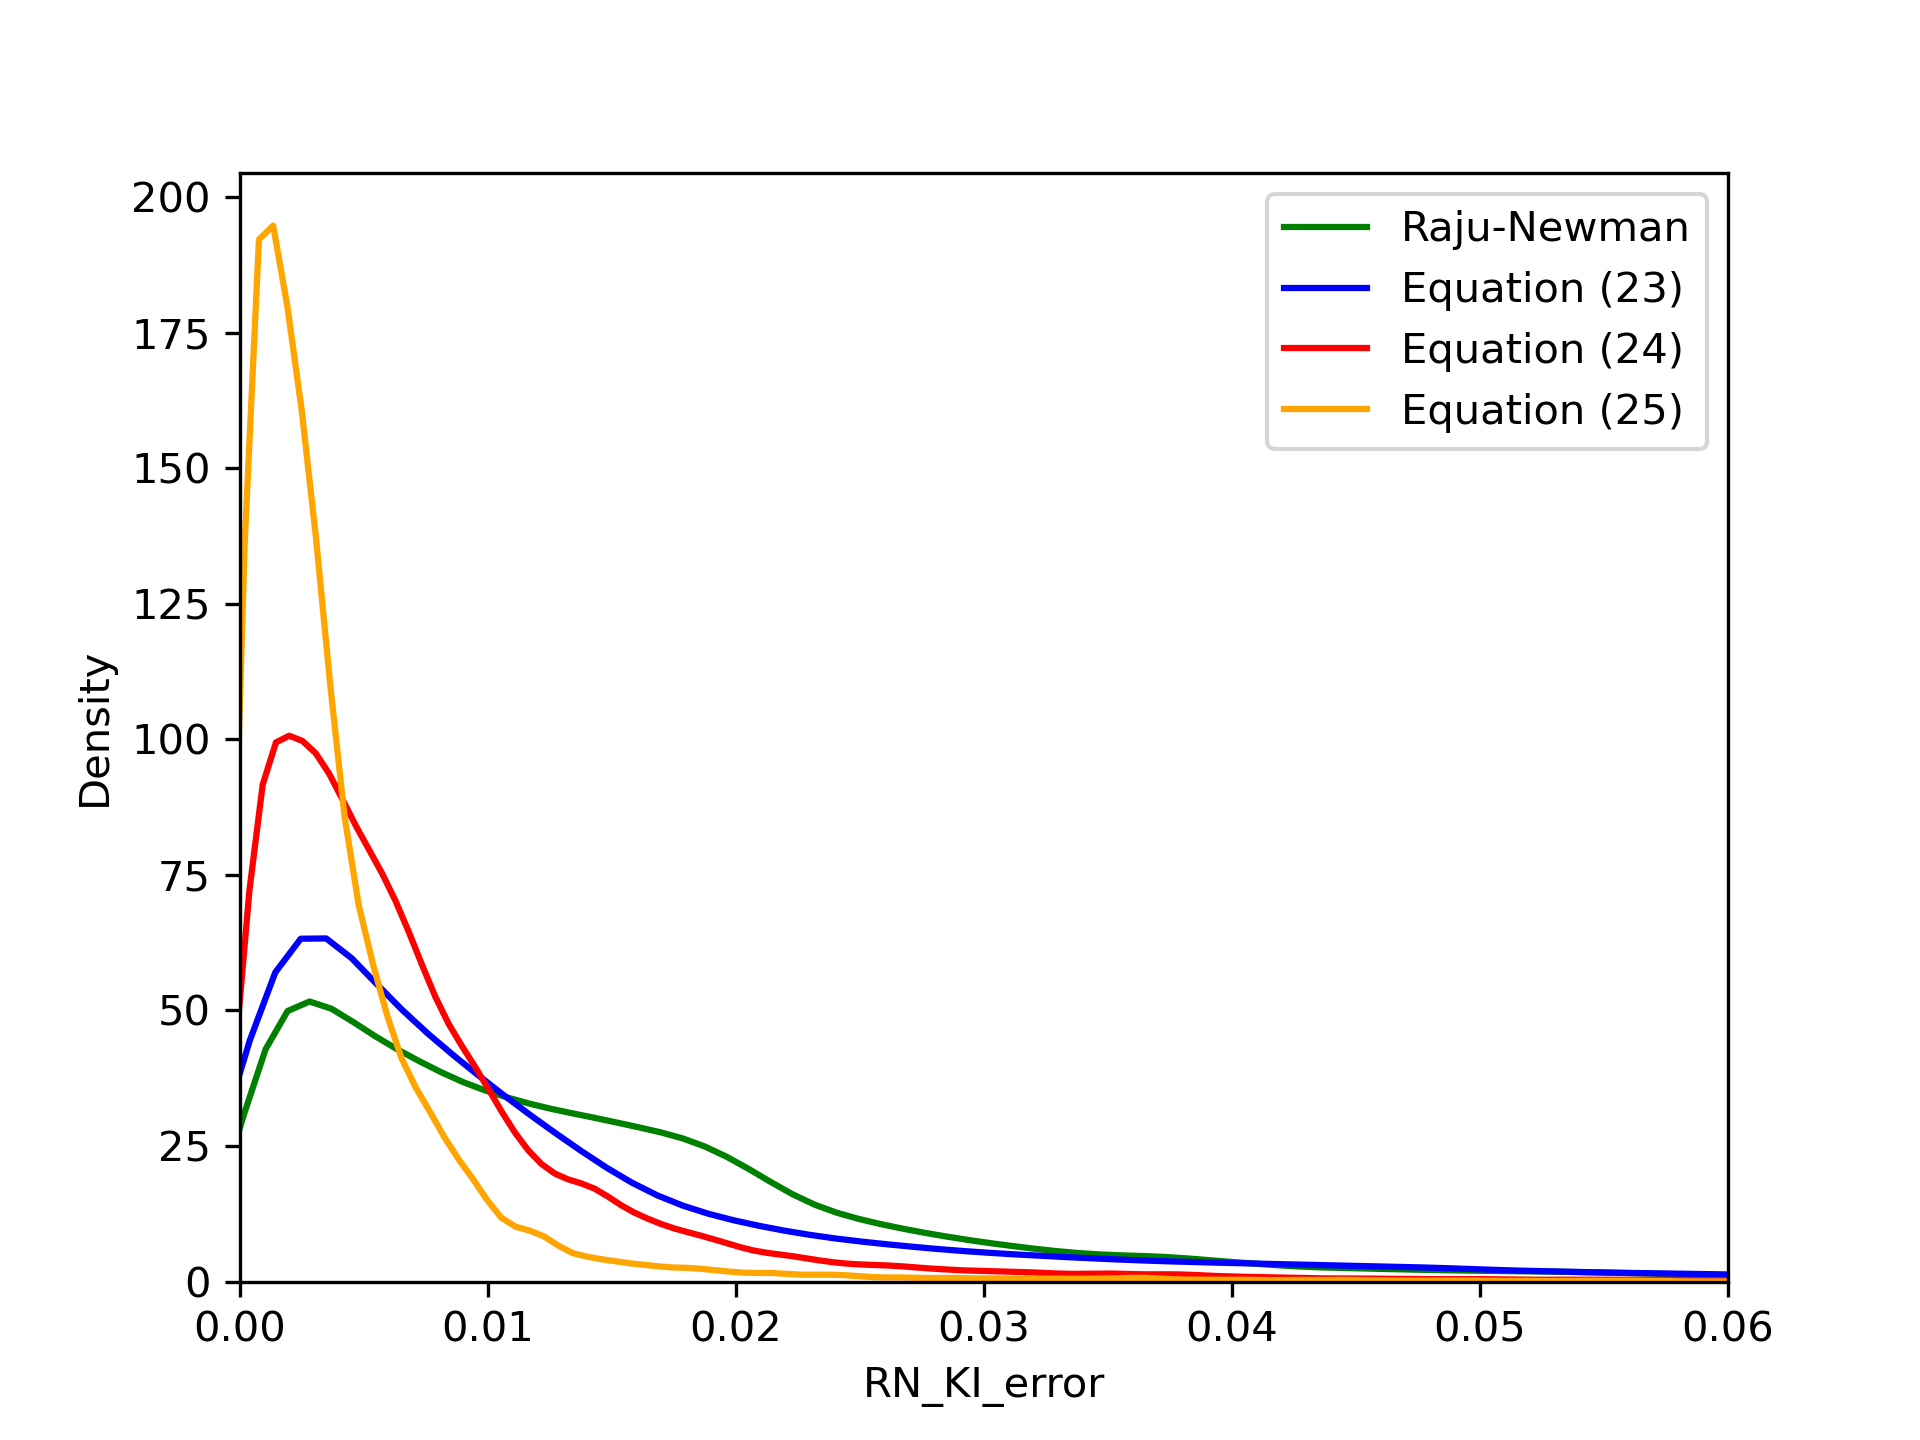
\includegraphics[width=3in]{Figures/kde_plot_everything.png} }}%
    \qquad
    \subfloat[\centering Parity plots]{{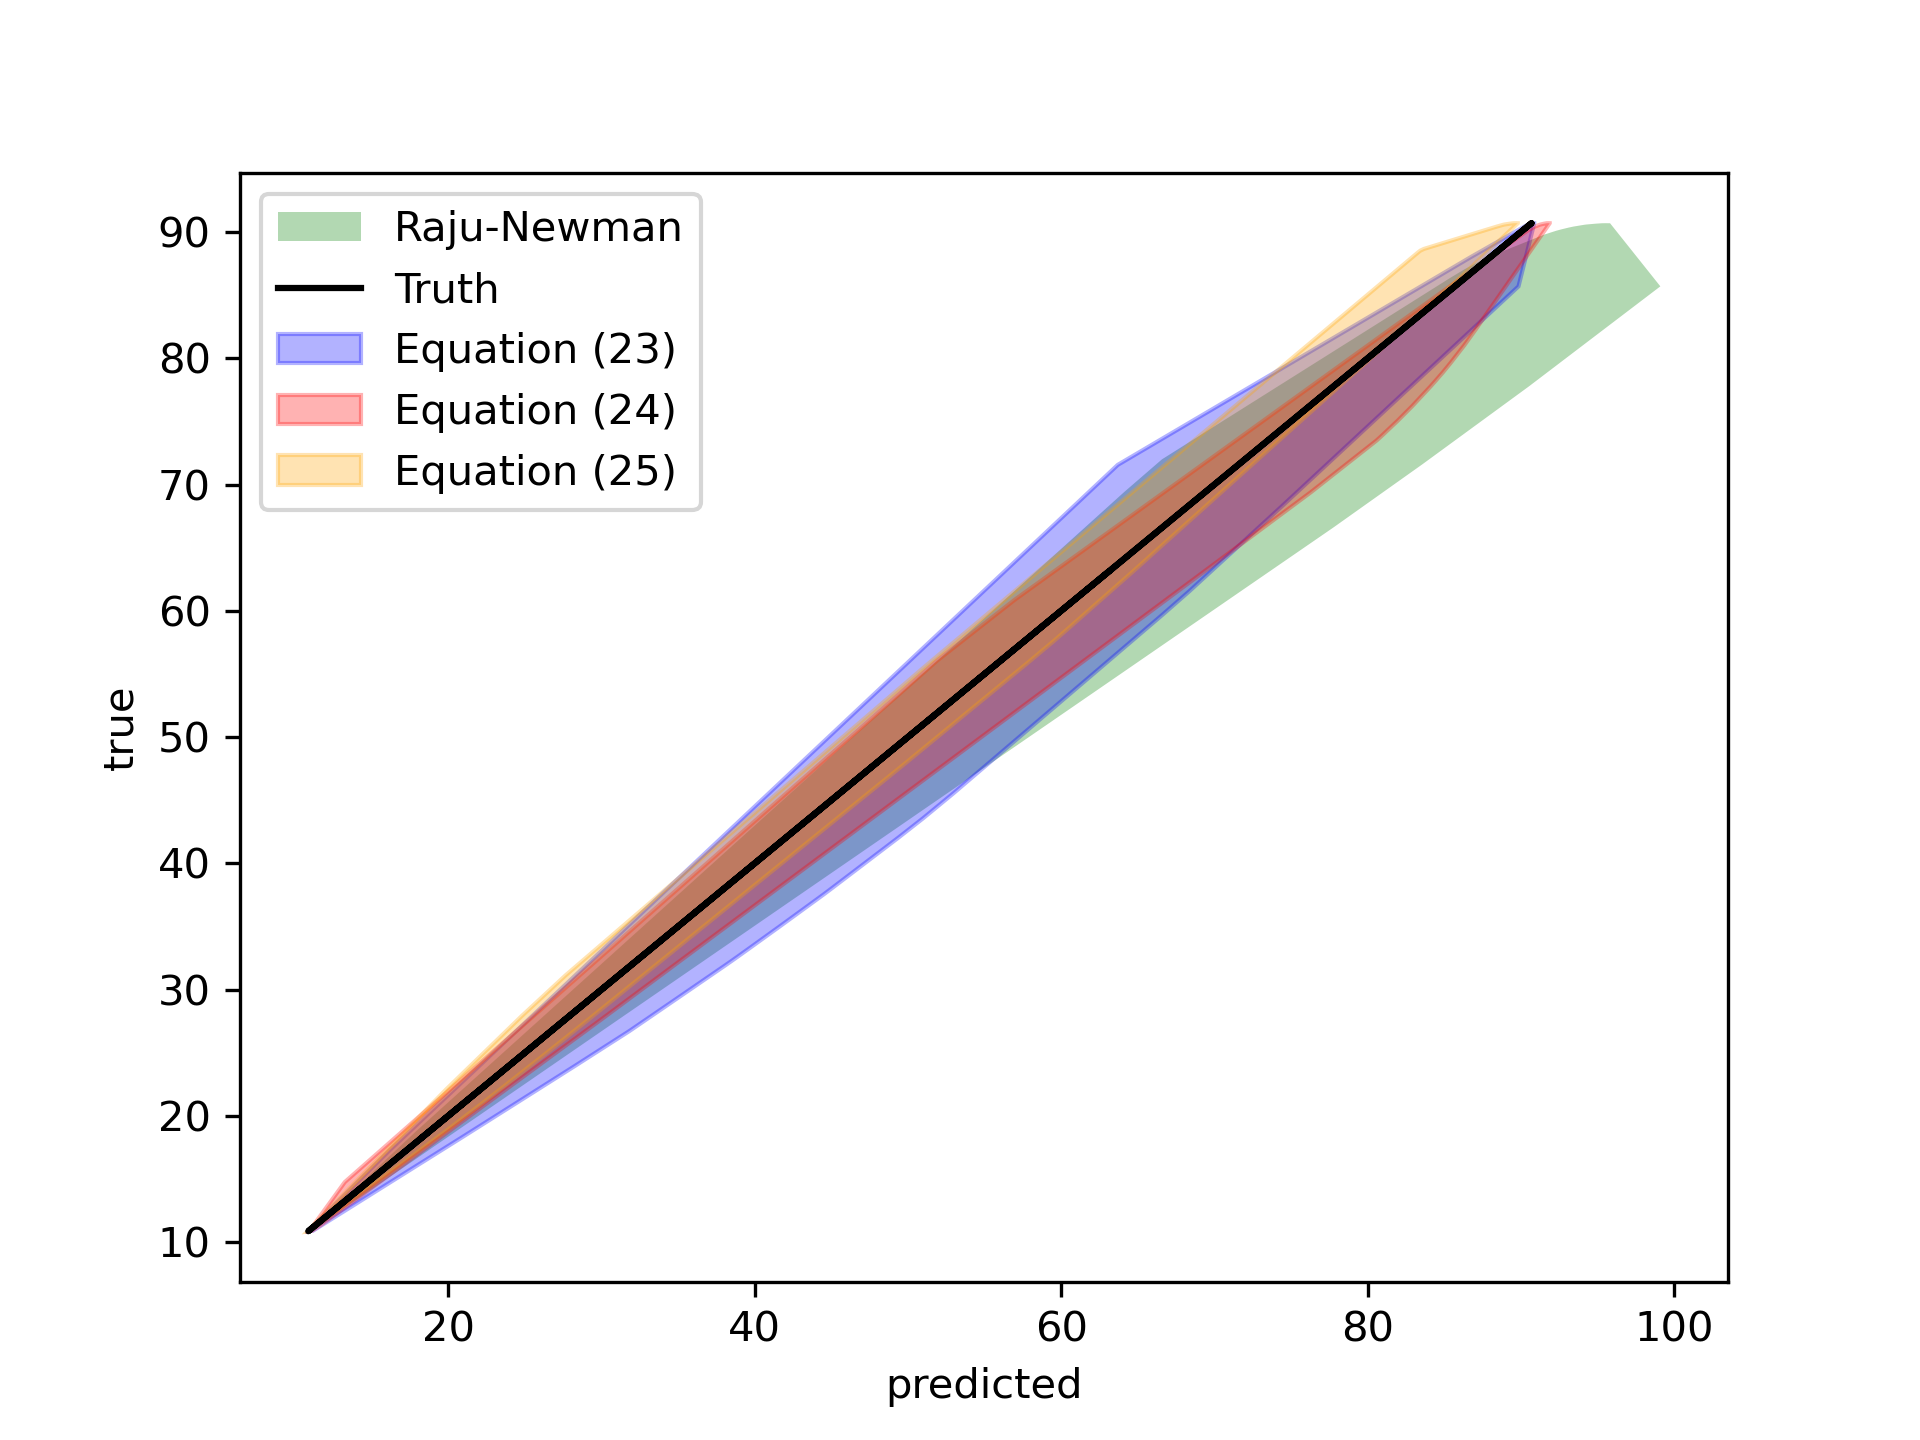
\includegraphics[width=3in]{Figures/parity_plot_everything.png} }}%
    \caption{(a) Density plot for the errors of each of the equations from the combined selection. (b) Parity plot with each of the different equations from the combined selection.}%
    \label{fig:combo_error_plots}%
\end{figure}


\begin{figure}
    \centering
    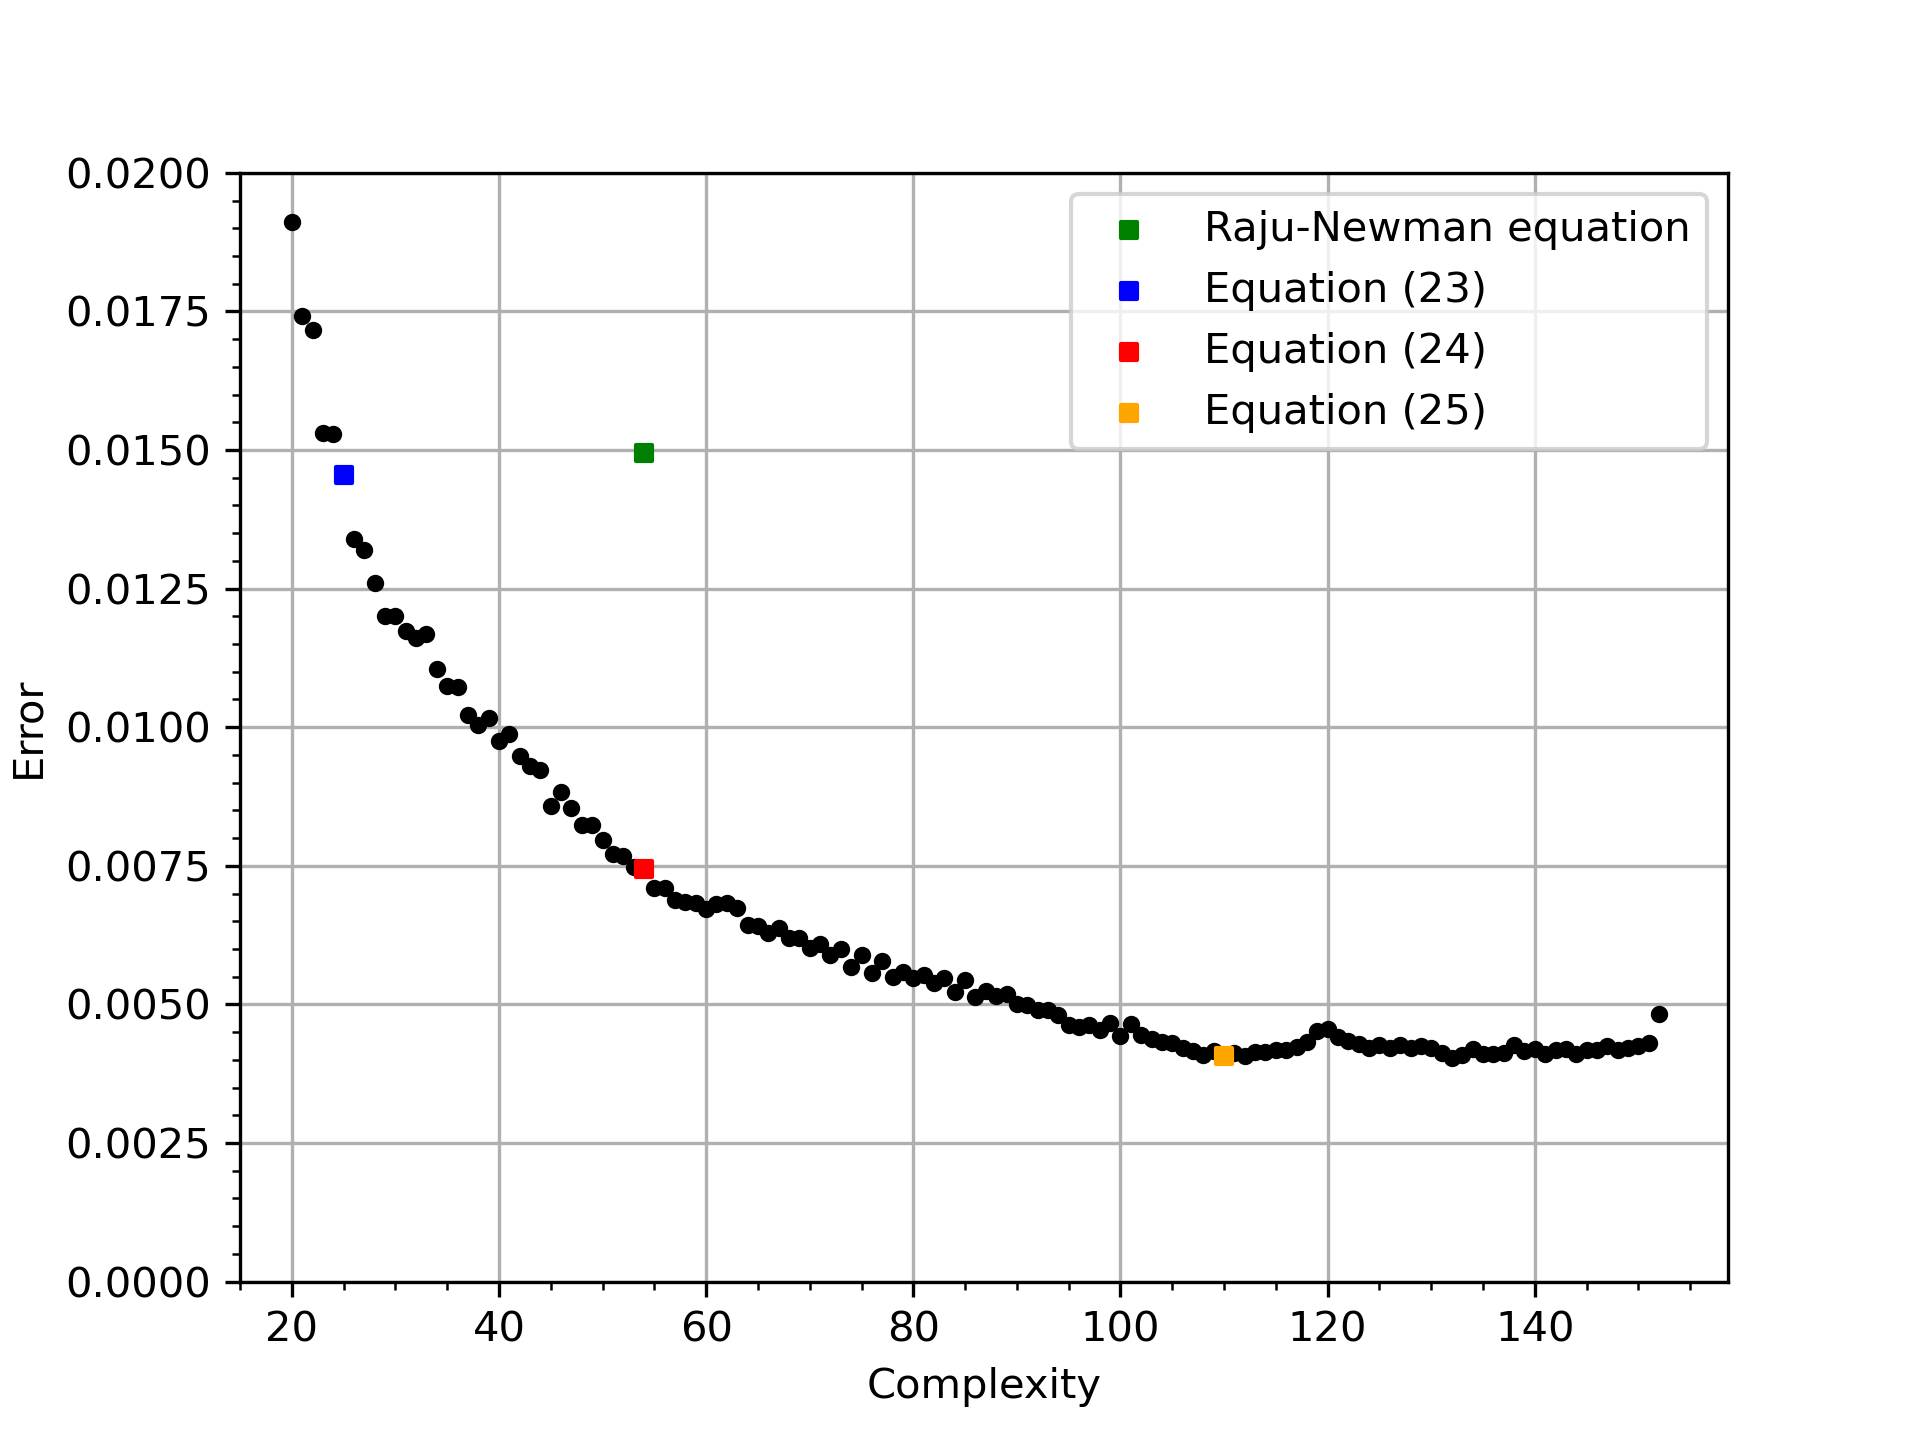
\includegraphics[width=5in]{Figures/perato_front_everything.png}
    \label{fig:perato_front_everything}
    \caption{Perato front for the models selected using all possible combinations.}
\end{figure}

\begin{figure}
    \centering
    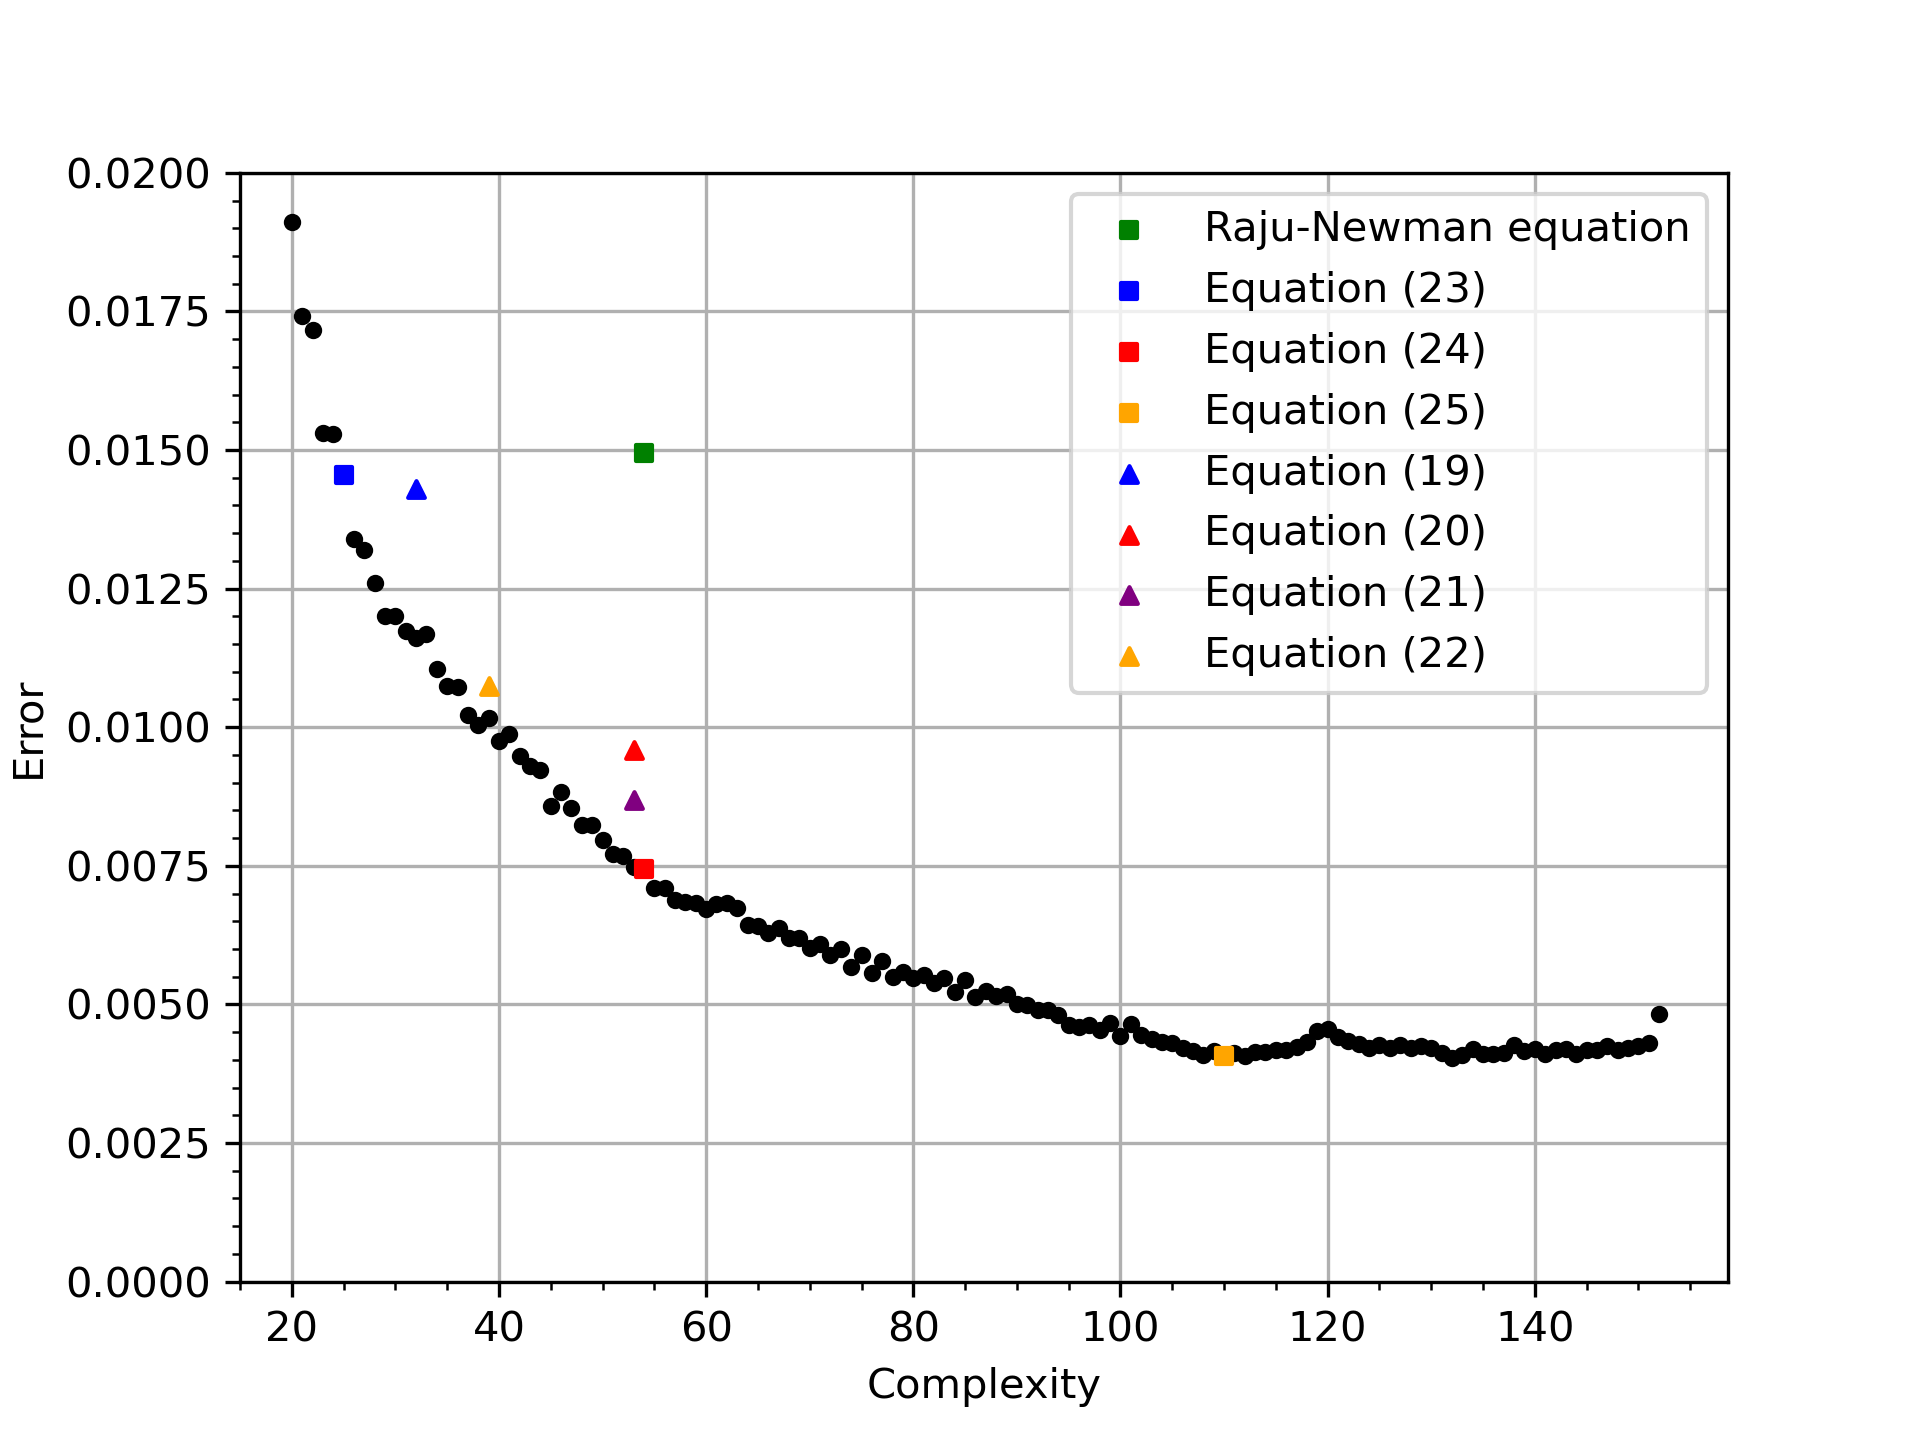
\includegraphics[width=5in]{Figures/perato_front_everything_and_more.png}
    \label{fig:perato_front_everything_ant_more}
    \caption{Perato front with all models the triangle models correspond to the models that were individually selected and the square models are the models selected using all possible combinations.}
\end{figure}

